%==============================================================================
% tento soubor pouzijte jako zaklad
% this file should be used as a base for the thesis
% Autoři / Authors: 2008 Michal Bidlo, 2016 Jaroslav Dytrych
% Kontakt pro dotazy a připomínky: dytrych@fit.vutbr.cz
% Contact for questions and comments: dytrych@fit.vutbr.cz
%==============================================================================
% kodovani: UTF-8 (zmena prikazem iconv, recode nebo cstocs)
% encoding: UTF-8 (you can change it by command iconv, recode or cstocs)
%------------------------------------------------------------------------------
% zpracování / processing: make, make pdf, make clean
%==============================================================================
% Soubory, které je nutné upravit: / Files which have to be edited:
%   projekt-20-literatura-bibliography.bib - literatura / bibliography
%   projekt-01-kapitoly-chapters.tex - obsah práce / the thesis content
%   projekt-30-prilohy-appendices.tex - přílohy / appendices
%==============================================================================
%\documentclass[]{fitthesis} % bez zadání - pro začátek práce, aby nebyl problém s překladem
%\documentclass[english]{fitthesis} % without assignment - for the work start to avoid compilation problem
%\documentclass[zadani]{fitthesis} % odevzdani do wisu - odkazy jsou barevné
%\documentclass[english,zadani]{fitthesis} % for submission to the IS FIT - links are color
%\documentclass[zadani,print]{fitthesis} % pro tisk - odkazy jsou černé
%\documentclass[zadani,cprint]{fitthesis} % pro barevný tisk - odkazy jsou černé, znak VUT barevný
%\documentclass[english,zadani,print]{fitthesis} % for the color print - links are black
%\documentclass[english,zadani,cprint]{fitthesis} % for the print - links are black, logo is color
% * Je-li práce psaná v anglickém jazyce, je zapotřebí u třídy použít
%   parametr english následovně:
%   If thesis is written in english, it is necessary to use
%   parameter english as follows:
%      \documentclass[english]{fitthesis}
% * Je-li práce psaná ve slovenském jazyce, je zapotřebí u třídy použít
%   parametr slovak následovně:
%   If the work is written in the Slovak language, it is necessary
%   to use parameter slovak as follows:
%      \documentclass[slovak]{fitthesis}
% * Je-li práce psaná v anglickém jazyce se slovenským abstraktem apod.,
%   je zapotřebí u třídy použít parametry english a enslovak následovně:
%   If the work is written in English with the Slovak abstract, etc.,
%   it is necessary to use parameters english and enslovak as follows:
      \documentclass[english,enslovak]{fitthesis}

% Základní balíčky jsou dole v souboru šablony fitthesis.cls
% Basic packages are at the bottom of template file fitthesis.cls
% zde můžeme vložit vlastní balíčky / you can place own packages here
\usepackage{epigraph}
\usepackage{graphicx}
% Kompilace po částech (rychlejší, ale v náhledu nemusí být vše aktuální)
% Compilation piecewise (faster, but not all parts in preview will be up-to-date)
\usepackage{subfiles}
\usepackage{tabto}
% Nastavení cesty k obrázkům
% Setting of a path to the pictures
%\graphicspath{{obrazky-figures/}{./obrazky-figures/}}
\graphicspath{{figures/}{../figures/}}

%---rm---------------
\renewcommand{\rmdefault}{lmr}%zavede Latin Modern Roman jako rm / set Latin Modern Roman as rm
%---sf---------------
\renewcommand{\sfdefault}{qhv}%zavede TeX Gyre Heros jako sf
%---tt------------
\renewcommand{\ttdefault}{lmtt}% zavede Latin Modern tt jako tt

% vypne funkci šablony, která automaticky nahrazuje uvozovky,
% aby nebyly prováděny nevhodné náhrady v popisech API apod.
% disables function of the template which replaces quotation marks
% to avoid unnecessary replacements in the API descriptions etc.
\csdoublequotesoff

% =======================================================================
% balíček "hyperref" vytváří klikací odkazy v pdf, pokud tedy použijeme pdflatex
% problém je, že balíček hyperref musí být uveden jako poslední, takže nemůže
% být v šabloně
% "hyperref" package create clickable links in pdf if you are using pdflatex.
% Problem is that this package have to be introduced as the last one so it
% can not be placed in the template file.
\ifWis
\ifx\pdfoutput\undefined % nejedeme pod pdflatexem / we are not using pdflatex
\else
  \usepackage{color}
  \usepackage[unicode,colorlinks,hyperindex,plainpages=false,pdftex]{hyperref}
  \definecolor{links}{rgb}{0.4,0.5,0}
  \definecolor{anchors}{rgb}{1,0,0}
  \def\AnchorColor{anchors}
  \def\LinkColor{links}
  \def\pdfBorderAttrs{/Border [0 0 0] }  % bez okrajů kolem odkazů / without margins around links
  \pdfcompresslevel=9
\fi
\else % pro tisk budou odkazy, na které se dá klikat, černé / for the print clickable links will be black
\ifx\pdfoutput\undefined % nejedeme pod pdflatexem / we are not using pdflatex
\else
  \usepackage{color}
  \usepackage[unicode,colorlinks,hyperindex,plainpages=false,pdftex,urlcolor=black,linkcolor=black,citecolor=black]{hyperref}
  \definecolor{links}{rgb}{0,0,0}
  \definecolor{anchors}{rgb}{0,0,0}
  \def\AnchorColor{anchors}
  \def\LinkColor{links}
  \def\pdfBorderAttrs{/Border [0 0 0] } % bez okrajů kolem odkazů / without margins around links
  \pdfcompresslevel=9
\fi
\fi
% Řešení problému, kdy klikací odkazy na obrázky vedou za obrázek
% This solves the problems with links which leads after the picture
\usepackage[all]{hypcap}

% Informace o práci/projektu / Information about the thesis
%---------------------------------------------------------------------------
\projectinfo{
  %Prace / Thesis
  project={BP},            %typ práce BP/SP/DP/DR  / thesis type (SP = term project)
  year={2018},             % rok odevzdání / year of submission
  date=\today,             % datum odevzdání / submission date
  %Nazev prace / thesis title
  title.cs={Portovanie Tang na OpenWrt},  % název práce v češtině či slovenštině (dle zadání) / thesis title in czech language (according to assignment)
  title.en={Porting Tang to OpenWrt}, % název práce v angličtině / thesis title in english
  %title.length={14.5cm}, % nastavení délky bloku s titulkem pro úpravu zalomení řádku (lze definovat zde nebo níže) / setting the length of a block with a thesis title for adjusting a line break (can be defined here or below)
  %Autor / Author
  author.name={Tibor},   % jméno autora / author name
  author.surname={Dudlák},   % příjmení autora / author surname
  %author.title.p={Bc.}, % titul před jménem (nepovinné) / title before the name (optional)
  %author.title.a={Ph.D.}, % titul za jménem (nepovinné) / title after the name (optional)
  %Ustav / Department
  department={UIFS}, % doplňte příslušnou zkratku dle ústavu na zadání: UPSY/UIFS/UITS/UPGM / fill in appropriate abbreviation of the department according to assignment: UPSY/UIFS/UITS/UPGM
  % Školitel / supervisor
  supervisor.name={Ondrej},   % jméno školitele / supervisor name
  supervisor.surname={Lichtner},   % příjmení školitele / supervisor surname
  supervisor.title.p={Ing.},   %titul před jménem (nepovinné) / title before the name (optional)
  %supervisor.title.a={Ph.D.},    %titul za jménem (nepovinné) / title after the name (optional)
  % Klíčová slova / keywords
  %keywords.cs={Sem budou zapsána jednotlivá klíčová slova v českém (slovenském) jazyce, oddělená čárkami.}, % klíčová slova v českém či slovenském jazyce / keywords in czech or slovak language
  keywords.cs={
    portovanie,
    Tang,
    server,
    Clevis,
    klient,
    Escrow,
    OpenWrt,
    operačný systém,
    vstavané zariadenie,
    šifrovanie,
    LUKS,
    pevný disk,
    diskový oddiel,
    šifrovací kľúč,
    automatizácia,
    cross-kompilácia,
    balíkový systém },
  keywords.en={
    porting,
    Tang,
    server,
    Clevis,
    client,
    Escrow,
    OpenWrt,
    operating system,
    embedded device,
    encryption,
    LUKS,
    hard drive,
    disk partition,
    encryption key,
    automation,
    cross-compiling,
    package system },
  % Abstrakt / Abstract
  %abstract.cs={Do tohoto odstavce bude zapsán výtah (abstrakt) práce v českém (slovenském) jazyce.}, % abstrakt v českém či slovenském jazyce / abstract in czech or slovak language
  %abstract.en={Do tohoto odstavce bude zapsán výtah (abstrakt) práce v anglickém jazyce.}, % abstrakt v anglickém jazyce / abstract in english
  abstract.cs={Hlavným cieľom tejto práce je sprístupnenie serveru Tang na vstavané zariadenia typu WiFi smerovač s plne modulárnym operačným systémom OpenWrt. Tým dosiahneme anonymnú správu šifrovacích kľúčov pre domáce siete a siete malých firiem. Preto táto práca popisuje problematiku šifrovania a jeho využitie na zabezpečenie pevného disku počítača. Oboznámuje čitateľa so štruktúrou šifrovaného diskového oddielu podľa LUKS špecifikácie na operačných systémoch typu Linux. Práca rozoberá možnosti automatizácie odomykania šifrovaných diskov použitím externého servera, ktorý vstupuje do procesu ako tretia strana. Sú v nej popísané princípy serverov Key Escrow a Tang. Dosiahnutie hlavného cieľa je možné vďaka procesu portovania a cross-kompilácie na platforme Linux.  Práca obsahuje zdokumentovaný postup prispievania zmien a novo vytvorených balíkov pre OpenWrt do príslušných Open Source projektov.},
  abstract.en={This thesis describes the encryption and its application to secure the computer's hard drive. It describes the structure of the encrypted disk's partition according to the LUKS specification on Linux operating systems. The thesis focus on describing possibilities of automating the disk decryption process using an external server that enters the process as a third party. It describes the principles of Key Escrow and Tang server. Steps required to compile and configure the Tang server are described too. Also described is Tang server's client -- Clevis. The main objective of this work was to port and document the process of porting the Tang server and its dependencies to OpenWrt system, described in this thesis too, which is designed for embedded devices such as WiFi routers. The thesis also includes a documented process of contributing changes and newly created OpenWrt packages to corresponding Open Source projects.},
  % Prohlášení (u anglicky psané práce anglicky, u slovensky psané práce slovensky) / Declaration (for thesis in english should be in english)
  declaration={Hereby I declare that this term project was prepared as an original author’s work under the supervision of Ing. Ondrej Lichtner.
  The supplementary information was provided by Jan Pazdziora, Ph. D.
  All the relevant information sources, which were used during preparation of this thesis, are properly cited and included in the list of references.
  },
%declaration={Prohlašuji, že jsem tuto bakalářskou práci vypracoval samostatně pod vedením pana X...
%Další informace mi poskytli...
%Uvedl jsem všechny literární prameny a publikace, ze kterých jsem čerpal.},
  %declaration={Hereby I declare that this bachelor's thesis was prepared as an original author’s work under the supervision of Mr. X
% The supplementary information was provided by Mr. Y
% All the relevant information sources, which were used during preparation of this thesis, are properly cited and included in the list of references.},
  % Poděkování (nepovinné, nejlépe v jazyce práce) / Acknowledgement (optional, ideally in the language of the thesis)
  acknowledgment={V této sekci je možno uvést poděkování vedoucímu práce a těm, kteří poskytli odbornou pomoc
(externí zadavatel, konzultant, apod.).},
  %acknowledgment={Here it is possible to express thanks to the supervisor and to the people which provided professional help
%(external submitter, consultant, etc.).},
  % Rozšířený abstrakt (cca 3 normostrany) - lze definovat zde nebo níže / Extended abstract (approximately 3 standard pages) - can be defined here or below
  %extendedabstract={Do tohoto odstavce bude zapsán rozšířený výtah (abstrakt) práce v českém (slovenském) jazyce.},
  faculty={FIT}, % FIT/FEKT/FSI/FA/FCH/FP/FAST/FAVU/USI/DEF
  faculty.cs={Fakulta informačních technologií}, % Fakulta v češtině - pro využití této položky výše zvolte fakultu DEF / Faculty in Czech - for use of this entry select DEF above
  faculty.en={Faculty of Information Technology}, % Fakulta v angličtině - pro využití této položky výše zvolte fakultu DEF / Faculty in English - for use of this entry select DEF above
  % department.cs={Ústav matematiky}, % Ústav v češtině - pro využití této položky výše zvolte ústav DEF nebo jej zakomentujte / Department in Czech - for use of this entry select DEF above or comment it out
  % department.en={Institute of Mathematics} % Ústav v angličtině - pro využití této položky výše zvolte ústav DEF nebo jej zakomentujte / Department in English - for use of this entry select DEF above or comment it out
}

% Rozšířený abstrakt (cca 3 normostrany) - lze definovat zde nebo výše / Extended abstract (approximately 3 standard pages) - can be defined here or above
%\extendedabstract{Do tohoto odstavce bude zapsán výtah (abstrakt) práce v českém (slovenském) jazyce.}

% nastavení délky bloku s titulkem pro úpravu zalomení řádku - lze definovat zde nebo výše / setting the length of a block with a thesis title for adjusting a line break - can be defined here or above
%\titlelength{14.5cm}


% řeší první/poslední řádek odstavce na předchozí/následující stránce
% solves first/last row of the paragraph on the previous/next page
\clubpenalty=10000
\widowpenalty=10000

\begin{document}
  % Vysazeni titulnich stran / Typesetting of the title pages
  % ----------------------------------------------
  \maketitle
  % Obsah
  % ----------------------------------------------
  \setlength{\parskip}{0pt}

  {\hypersetup{hidelinks}\tableofcontents}

  % Seznam obrazku a tabulek (pokud prace obsahuje velke mnozstvi obrazku, tak se to hodi)
  % List of figures and list of tables (if the thesis contains a lot of pictures, it is good)
  \ifczech
    \renewcommand\listfigurename{Seznam obrázků}
  \fi
  \ifslovak
    \renewcommand\listfigurename{Zoznam obrázkov}
  \fi
  % \listoffigures

  \ifczech
    \renewcommand\listtablename{Seznam tabulek}
  \fi
  \ifslovak
    \renewcommand\listtablename{Zoznam tabuliek}
  \fi
  % \listoftables

  \ifODSAZ
    \setlength{\parskip}{0.5\bigskipamount}
  \else
    \setlength{\parskip}{0pt}
  \fi

  % vynechani stranky v oboustrannem rezimu
  % Skip the page in the two-sided mode
  \iftwoside
    \cleardoublepage
  \fi

  % Text prace / Thesis text
  % ----------------------------------------------
  \chapter{Introduction}\label{introduction}
\epigraph{\it We spend our time searching for security, and hate it when we get it.}{{John Steinbeck}\cite{quote}}

Nowadays, the whole world uses information technologies to communicate and to spread knowledge in form of bits to the other people.
But there are pieces of personal information such as photos from family vacation, videos of our children as they grow, contracts, testaments which we would like to protect.

{\it Encryption}, as described in chapter \ref{encryption} How we use Encryption, protects our data and privacy even when we do not realize that.
An unauthorized party may be able to access secured data but will not be able to read the information from it without the proper key.
With an increasing number of encryption keys to store and protect, there might be necessary to consider using Key management server.
One of the possible solutions for persistent Key management is to deploy {\it key escrow} server described in section \ref{escrow}Key Escrow.
Another solution is server {\it Tang}, which principles are mentioned in section \ref{tang} Tang server.

Tang is completely anonymous key recovery service aiming to solve an early boot decryption of the system volumes encrypted with LUKS specification described in section \ref{LUKS_disk} Disk encryption with LUKS.
In contrast to Key Escrow server, Tang does not know any key.
It only provides mathematical operation for its clients to recover them.

The goal of this bachelor thesis is to port the {\it Tang} server, and its dependencies listed in section \ref{dependencies} to the OpenWrt system.
{\it OpenWrt}, characterized in section \ref{owrt} OpenWrt system, is Linux based operating system for {\it embedded} devices such as Wireless routers.
Porting packages for the OpenWrt as described in chapter\ref{porting} Software portability is done with cross-compilation tools available from OpenWrt's buildroot.

The process of porting missing dependecies for the Tang server is described in chapter \ref{satisfy_dependencies} Porting the dependencies.
Work required for the Tang itself is divided into chapters \ref{porting-tang} Porting Tang and \ref{config} Tang on OpenWrt.

Section \ref{limitations} Tang's limitations sums up not only the limitations that are present on OpenWrt platform but also a limitation that was discovered while testing solution.

With accomplishing thesis goal, we will be able to automatize process of unlocking encrypted drives on our private home or small office network, therefore securing our data stored on personal computer's hard drive and/or NAS (Network-attached storage) server if it is stolen.
There will be no need for any decryption or even Key Escrow server but the {\it OpenWrt} device running the {\it Tang} server itself only.

  \chapter{How We Use Encryption}\label{encryption}

We may not realize this, but we use encryption every day.
The purpose of encryption is to keep us safe when we are browsing the Internet or just storing our sensitive information on digital media.
In general encryption is used to secure our data, whether transmitted around the Internet or stored on our hard drives, from being compromised.
Encryption protects us from many threats.

It protects us from identity theft.
Our personal information stored all over governmental authorities should be secured with it.
Encryption takes care for not revealing sensitive information about ourselves, to protect our financial details, passwords along with others, mainly when we bank online.

It looks after our conversation privacy, protecting our cell phone conversations from eavesdroppers and our online chatting with acquaintances or colleagues.
It also allows attorneys to communicate privately with their clients and it aims to secure communication between investigation bureaus to exchange sensitive information about lawbreakers.

If we encrypt our laptop or desktop computer's hard drive, encryption protects our data in case the computer or hard drive is stolen.



\section{Encryption and Security}

Security is not binary; it is a sliding scale of risk management.
People are used to mark things, for example good and bad, expensive, and cheap.
But we know that people may differ on image/sense.
For example, there is no such thing as line or sign which tells us that this part of town is secure, and this is not.
The way we reason about security is by studying environment, entering or observing it, and we begin to decide whether it is secure or not.
Encryption, on its own, might not be enough to make our data or infrastructure secure but is definitely a critical aspect of security.

Companies define their own security strategies which may include encryption or may not at all.
Security strategies rely on company's needs or will to take risks.

According to 2016 Global Encryption Trends Study, independently conducted by the Ponemon Institute, the enterprise-wide encryption increased from 15 percent in February 2006 to 41 percent in February 2017.
Also, the ratio of companies with no encryption strategy at all decreased from 37 to 14 percent in these years.
More than 60 percent of companies are using extensively deployed encryption technologies to encrypt mostly databases, infrastructure and laptop hard drives \cite{Thales}.

Passwords are the most common authentication method used for accessing computer systems, files, data, and networks.
As stated in article {\it Solid IT control hygiene} \cite{Perry2017}\label{rotation}, it is important to keep changing them in reasonable time and keep them secret to others.
Still, no matter the company's security strategy, we keep seeing them on monitors or desktops written on sticky notes, and this is absolutely not secure.
In fact, users are the most vulnerable part of securing our systems.
To aid their memory, users often include part of a phone number, family name, Social Security number, or even birth date in their passwords \cite{pwdsec}.
They choose cryptographically weak passwords, dictionary words, which are easy to remember but also easy to guess or to break with brute-force attacks in short period of time.
According to Splash Data, a supplier of security applications, the most common user selected password in the year 2016 was “123456”.
They claim that people continue to put themselves at risk for hacking and identity theft by using weak, easily guessable passwords.
To create strong password, we may follow any trustworthy guide\footnote{https://www.wikihow.com/Create-a-Secure-Password} on the Internet.
More secure way to create passwords would be to generate cryptographically stronger cipher and use it as a password.
The only disadvantage is that it is hard to remember \cite{splashdata}.



\section{Hard Drive Encryption}

It all starts, as mentioned, with desire to keep our data to ourselves and as a secret to others.
More often than not, these secrets are stored on our hard drives.

Hard drive encryption is a technology provided by software performing sophisticated mathematical functions or hardware that encrypts the data stored on a hard drive or a disk volume.
This technology is used to prevent unauthorized access by unauthorized persons or service to an encrypted data storage without possession of the appropriate key or password.
Encrypting the hard drive means providing another layer of security against hackers and other online threats.

To protect secret data, we usually encrypt this data by using an “encryption key” -- see Figure \ref{fig_encdata} Hard drive encryption in a nutshell.
\begin{figure}[h]
    \centering
    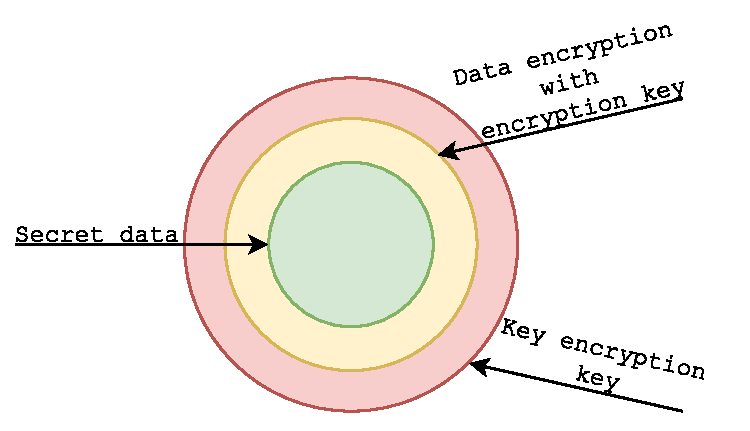
\includegraphics[scale=0.7]{figures/HowWeEncryptData.pdf}
    \caption{Hard Drive Encryption in a Nutshell}
    \label{fig_encdata}
\end{figure}
Every encryption key should be unpredictable and unique set of bits able to “scramble” data in a way that it should be impossible to recover data without the key.
To satisfy this need, encryption keys are generated by specialized algorithms such as AES (Advanced Encryption Standard\footnote{https://en.wikipedia.org/wiki/Symmetric-key\_algorithm\#Implementations}) for symmetric keys and RSA (Rivest–Shamir–Adleman\footnote{https://en.wikipedia.org/wiki/Public-key\_cryptography}) for asymmetric.
Changing encryption key implies that all the data needs to be decrypted with the old key and re-encrypted with the new one, every time the old key is compromised or a change is required.
To avoid time-consuming re-encryption whenever key change occurs, the encryption key is then wrapped by the key encryption key.

Key encryption key is mostly generated using the user-provided password.
This key encryption key is then used to encrypt the encryption key which does the actual data encryption.
Again, the most insecure thing in this key hierarchy would be the user-provided password which we can easily replace with using only cryptographically stronger key.
This principle has at least two advantages.
Changing the key encryption key does not affect encrypted data, and key can be changed whenever the user desires to, and redistributed to all users or services that are supposed to decrypt this data, giving access to the encryption key.

Hard drive can be encrypted as whole or per partition.
Full disk encryption is done in a way that all content on the hard drive except MBR (Master Boot Record) is encrypted.
Encrypting MBR would make it impossible to start boot sequence of operating system.
Boot sequence would prompt the user for key encryption key in order to load the operating system from encrypted storage.

This could disrupt our daily workflow and might be the reason why most of us do not use hard drive encryption, even when we know it will protect our data.
There is a way to automate the hard drive unlocking on early boot with a help from key management system.
We can get the key encryption key from some remote system, the Escrow server mentioned in section \ref{escrow}, or recover it with Tang described in chapter \ref{tang}.
Before that, let us have a look on most common hard drive encryption implementations.



\subsection{Bit Locker}
BitLocker is a closed source, full disk data protection feature that integrates with the operating system Windows Vista and later.
It is designed to protect data by providing encryption for entire volumes and addresses the threats of data theft or exposure from lost, stolen, or inappropriately decommissioned computers.
By default, it uses the AES encryption algorithm in cipher block chaining (CBC) or XTS mode with a 128-bit or 256-bit key.
CBC is not used over the whole disk; it is applied to each individual sector \cite{bitlocker}.



\subsection{LibreCrypt}

LibreCrypt is a {\it LUKS} (Linux Unified Key Setup-on-disk-format) compatible open source “on-the-fly” transparent disk encryption software written mostly in Pascal programming language.
This project is based on original FreeOTFE project by Sarah Dean renamed in version 6.2 to LibreCrypt and supports both 32 and 64 bit Windows.
LibreCrypt is easy to use even for inexperienced user through its GUI (Graphical User Interface) with support of many languages.

LibreCrypt supports many ciphers including AES (up to 256 bit), Twofish\footnote{https://en.wikipedia.org/wiki/Twofish} (up to 256 bit), Blowfish\footnote{https://en.wikipedia.org/wiki/Blowfish\_(cipher)} (up to 448 bit), Serpent\footnote{https://en.wikipedia.org/wiki/Serpent\_(cipher)} (up to 256 bit).
It can create “virtual disks” on our computer and anything written to these disks is automatically encrypted before being stored on our computer’s hard drive\cite{FreeOTFE}.

Unfortunately this project seems to be abandoned by its developer.
The source code of LibreCrypt is available at GitHub.
\begin{lstlisting}[columns=fixed,basicstyle=\ttfamily\footnotesize,tabsize=4,backgroundcolor=\color{yellow!10}]
https://github.com/t-d-k/LibreCrypt
\end{lstlisting}



\subsection{Dm-crypt}\label{dm-crypt}

The device-mapper crypt target ({\it dm-crypt}) provides transparent encryption of block devices using the kernel crypto API (Application programming interface) supporting ciphers and digest algorithms via standard kernel modules.
Device-mapper is a part of the Linux kernel that provides a generic way to create virtual layers of block devices, for example LVM (Logical Volume Manager) logical volumes.

In Fedora and Red Hat Enterprise Linux distributions, user-space interaction with {\it dm-crypt} is managed by a tool called {\tt cryptsetup}, which uses the device-mapper infrastructure to setup and operate on encrypted block devices.
With modern versions of {\tt cryptsetup} (i.e., since ~2006), encrypted block devices can be created in two main formats, plain {\it dm-crypt} format or the extended {\it LUKS} format.

Plain format has no meta-data on disk.
When using any such encrypted device, all the necessary parameters must be passed to {\tt cryptsetup} from the command line, otherwise it uses the defaults, which will only succeed if the device was created using default settings.
It derives (generates) the encryption key from the pass-phrase provided and then uses that to decrypt or encrypt the sectors of the device, with a direct 1:1 mapping between encrypted and decrypted sectors.

In contrast to previous Linux disk encryption solutions, {\it LUKS} stores all necessary setup information in the partition header, enabling the user to transport or migrate their data more easily.



\section{Disk Encryption with LUKS}\label{LUKS}

{\it LUKS} (Linux Unified Key Setup-on-disk-format) is a platform-independent disk encryption specification.
{\it LUKS} was created by Clemens Fruhwirth in 2004 and was originally intended for Linux distributions only.
It provides a standard on-disk-format for hard disk encryption, which facilitates compatibility among Linux distributions and provides secure management of multiple user passwords.

Referential implementation of {\it LUKS} is using a device-mapper crypt target ({\it dm-crypt}) subsystem for bulk data encryption.
This subsystem is not particularly bound to {\it LUKS} and can be used for plain format encryption as mentioned in subsection \ref{dm-crypt}.

It is important for us to know this specification a little more due to working with Linux distribution and the implementation of the Tang server.

The advantages of {\it LUKS} over plain {\it dm-crypt} are better usability: automatic configuration of non-default crypto parameters and the ability to add, change, and remove multiple pass-phrases.
Additionally, {\it LUKS} offers defenses against low-entropy pass-phrases with salting and iterated PBKDF2\footnote{https://www.ietf.org/rfc/rfc2898.txt} (Password-Based Key Derivation Function 2) pass-phrase hashing\cite{RFC2898}.
With {\it LUKS}, encryption keys are always generated by the kernel RNG (Random number generator); in contrast to plain {\it dm-crypt} where one can choose a simple dictionary word and have an encryption key derived from that.
One disadvantage of using {\it LUKS} over plain is that it is readily obvious there is encrypted data on disk; the other is that damage to the header or key slots usually results in permanent data loss.
To mitigate this risk the Backup of the {\it LUKS} header is the best option \cite{fruhwirth2005luks}.



\subsection{Creating LUKS Volume}

Creating a {\it LUKS} volume with the {\tt cryptsetup} tool is easy.
On Fedora system it can be installed using command:
\begin{lstlisting}[columns=fixed,basicstyle=\ttfamily\footnotesize,tabsize=4,backgroundcolor=\color{yellow!10}]
# dnf install cryptsetup
\end{lstlisting}
Run this command with root privileges.
After installation succeeds choose a partition to encrypt.
For demonstration, we will encrypt the {\tt /dev/xvdc} patrtition using:
\begin{lstlisting}[columns=fixed,basicstyle=\ttfamily\footnotesize,tabsize=4,backgroundcolor=\color{yellow!10}]
# cryptsetup -y -v luksFormat /dev/xvdc
WARNING!
========
This will overwrite data on /dev/xvdc irrevocably.

Are you sure? (Type uppercase yes): YES
Enter LUKS passphrase:
Verify passphrase:
Command successful.
\end{lstlisting}
But converting existing non-encrypted disk to have full disk encryption if the system is already installed might be quite tough.
Hard drive partition must contain the {\it LUKS} header just before the encrypted data.
Let us sum up the easier way first.

In case we have not installed our Linux operation system yet, we could simply select an option in time of installation.
Then the installation wizard will most likely ask for pass phrase -- the key encryption key.
To demonstrate this, screen shots with Fedora 28 system installation can be found in appendix \ref{luksinstall}.

If we have already system installed with lots of data on partition, process will probably last longer and the procedure will be more complex.
There is no way we can encrypt the whole system disk with {\it LUKS} without unmounting a partition to encrypt.
For this purpose {\it luksipc}, the LUKS In-Place Conversion Tool, was developed.
Steps to encrypt a disk using {\it luksipc} are in the appendix \ref{luksipc}.



\subsection{LUKS drive structure}

The structure of {\it LUKS} partition is shown in Figure \ref{fig_luksvol} LUKS volume structure for a demonstration.
At the the beginning of the device the {\it LUKS} format uses a meta-data header, also marked as {\it phdr}, and 8 key slot areas.
After header, there is a section with bulk data, which is encrypted with the encryption key.
\begin{figure}[h]
    \centering
    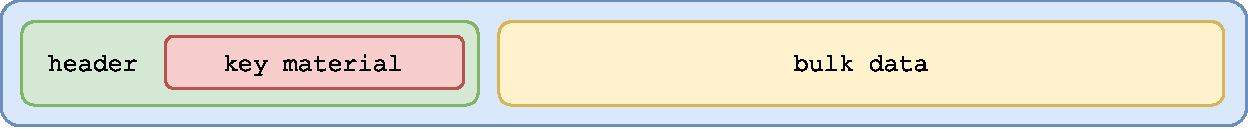
\includegraphics[scale=0.7]{figures/LUKSdrive.pdf}
    \caption{LUKS Volume Structure}
    \label{fig_luksvol}
\end{figure}
Header contains information about the cipher used, cipher mode, the key length, a uuid, and a encryption key check-sum.
The pass-phrases stored in the key slots, which structure is shown on Figure \ref{fig_luksslot} LUKS Key Slot, are used to decrypt a single key encryption key that is stored in the anti-forensic stripes.
Anti-forensic data storage, as described in article {\it LUKS On-Disk Format Specification Version 1.1} \cite{fruhwirth2005luks}, is a feature specially developed for {\it LUKS} by Clemens Fruhwirth.
The idea of anti-forensic information splitting in {\it LUKS} is to enlarge the size of every storage region for the encryption key encrypted with one of the user key encryption keys such that all parts of this storage region are required in order to recover the encrypion key.

\begin{figure}[h]
    \centering
    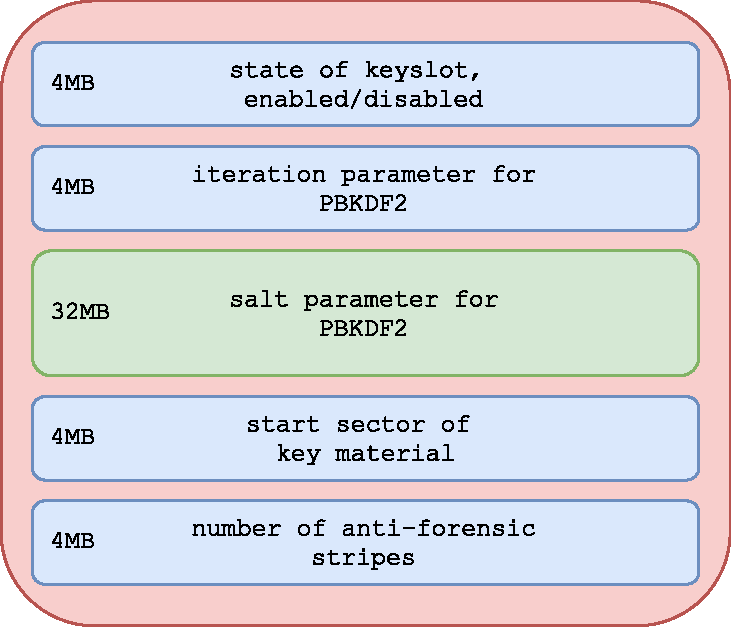
\includegraphics[scale=0.6]{figures/LUKSkeyslot.pdf}
    \caption{LUKS Key Slot}
    \label{fig_luksslot}
\end{figure}
Every key slot is associated with a key material section after the header.
When a key slot is active, the key slot stores an encrypted copy of the encryption key in its key material section.
This encrypted copy is locked by a user password or cipher.
Supplying this user password unlocks the decryption for the key material, which stores the encryption key.



\subsection{Managing LUKS volume}\label{manageLUKS}

To demonstrate {\it LUKS} volume management let us shot steps that can be used on our Fedora 27 system.
For this demonstration we will use tools available for Fedora 27 such as:\\
\begin{itemize}
    \item parted-3.2-28.fc27.x86\_64
    \item cryptsetup-1.7.5-3.fc27.x86\_64
\end{itemize}
To list hard drives for our system we will use the {\tt parted} tool:
\begin{lstlisting}[columns=fixed,basicstyle=\ttfamily\footnotesize,tabsize=4,backgroundcolor=\color{yellow!10}]
# parted -l
Model: NVMe Device (nvme)
Disk /dev/nvme0n1: 256GB
Sector size (logical/physical): 512B/512B
Partition Table: msdos
Disk Flags:

Number  Start   End     Size    Type     File system  Flags
 1      1049kB  1075MB  1074MB  primary  ext4         boot
 2      1075MB  256GB   255GB   primary
\end{lstlisting}
The output shows that on our system we have installed an NVMe (NVM Express) volume\footnote{https://en.wikipedia.org/wiki/NVM\_Express} using the msdos, therefore MBR partition table.
The NVMe is a specification for accessing SSDs attached through the PCI Express bus.
Our SSD drive has two partitions the first is a boot partition and second should be our {\it LUKS} partition.
To find out if the second partition is {\it LUKS} volume, we will use cryptsetup tool with option {\it isLuks}:
\begin{lstlisting}[columns=fixed,basicstyle=\ttfamily\footnotesize,tabsize=4,backgroundcolor=\color{yellow!10}]
# cryptsetup isLuks /dev/nvme0n1p1 -v
Device /dev/nvme0n1p1 is not a valid LUKS device.
Command failed with code 22: Invalid argument
\end{lstlisting}
Unless the {\tt -v} option is used, this command produces no output.
The actual result of the command is returned as an exit code.
The output shown reflects that our first partition is not a valid {\it LUKS} volume.
This is expected behavior, encrypting the boot partition would make it impossible for the system to boot.
\begin{lstlisting}[columns=fixed,basicstyle=\ttfamily\footnotesize,tabsize=4,backgroundcolor=\color{yellow!10}]
# cryptsetup isLuks /dev/nvme0n1p2 -v
Command successful.
\end{lstlisting}
At this point, we have successfully identified the {\it LUKS}volume.
To dump the header information of this {\it LUKS} volume, {\tt cryptsetup} option {\it luksDump} can be used:
\begin{lstlisting}[columns=fixed,basicstyle=\ttfamily\footnotesize,tabsize=4,backgroundcolor=\color{yellow!10}]
# cryptsetup luksDump /dev/nvme0n1p2
LUKS header information for /dev/nvme0n1p2

Version:		1
Cipher name:	aes
Cipher mode:	xts-plain64
Hash spec:		sha256
Payload offset:	4096
MK bits:		512
MK digest:		85 b3 b9 71 b6 b7 51 18 60 39 78 db ac e8 82 97 0c 7b a2 3e
MK salt:		0d 22 53 83 56 0d a0 70 25 c2 bf fe 75 40 71 a9
				75 f1 ae a3 67 e5 b2 a5 14 85 39 1d c6 74 00 a8
MK iterations: 	52625
UUID:          	267c308e-5d64-4acf-abf2-f6e224e8febf

Key Slot 0: ENABLED
	Iterations:				415583
	Salt:		3e f9 7d 3b b6 08 60 9a eb dc 52 bb 8e 21 eb bf
				b9 4d 80 a4 70 2d 4e 97 8e 47 c1 a3 04 45 74 d4
	Key material offset:	8
	AF stripes:				4000
Key Slot 1: DISABLED
Key Slot 2: DISABLED
Key Slot 3: DISABLED
Key Slot 4: DISABLED
Key Slot 5: DISABLED
Key Slot 6: DISABLED
Key Slot 7: DISABLED
\end{lstlisting}
From the listing we can assume that {\tt /dev/nvme0n1p2} has one key encryption key in key slot 0 and has other 7 slots (1-7) disabled.
The advantage of {\it LUKS} is that if a team or group of up to eight people has to work with a common encrypted volume, each team member may use their own password.
New user keys may be added to the encrypted volume and old user keys may be removed.
To add a new key, we will use {\tt cryptsetup} with option {\it luksAddKey} as shown:
\begin{lstlisting}[columns=fixed,basicstyle=\ttfamily\footnotesize,tabsize=4,backgroundcolor=\color{yellow!10}]
# cryptsetup luksAddKey  /dev/nvme0n1p2
Enter any existing passphrase:
Enter new passphrase for key slot:
Verify passphrase:
\end{lstlisting}
The {\tt cryptsetup} will derive the key encryption key from this passphrase and bind it to the first available key slot in {\it LUKS} header.
The dump of header will now contain information similar to the exhibit below:
\begin{lstlisting}[columns=fixed,basicstyle=\ttfamily\footnotesize,tabsize=4,backgroundcolor=\color{yellow!10}]
# cryptsetup luksDump /dev/nvme0n1p2
LUKS header information for /dev/nvme0n1p2

Version:		1
Cipher name:	aes
Cipher mode:	xts-plain64
Hash spec:		sha256
Payload offset:	4096
MK bits:		512
MK digest:		85 b3 b9 71 b6 b7 51 18 60 39 78 db ac e8 82 97 0c 7b a2 3e
MK salt:		0d 22 53 83 56 0d a0 70 25 c2 bf fe 75 40 71 a9
				75 f1 ae a3 67 e5 b2 a5 14 85 39 1d c6 74 00 a8
MK iterations: 	52625
UUID:			267c308e-5d64-4acf-abf2-f6e224e8febf

Key Slot 0: ENABLED
	Iterations:				415583
	Salt:		3e f9 7d 3b b6 08 60 9a eb dc 52 bb 8e 21 eb bf
				b9 4d 80 a4 70 2d 4e 97 8e 47 c1 a3 04 45 74 d4
	Key material offset:	8
	AF stripes:				4000
Key Slot 1: ENABLED
	Iterations:				1247257
	Salt:		44 48 92 df 29 8a df 81 f6 44 f8 66 c5 c2 32 49
				23 76 8a 37 48 85 33 2a 29 10 d8 cc 8f 45 0a 46
	Key material offset:	1520
	AF stripes:				4000
Key Slot 2: DISABLED
Key Slot 3: DISABLED
Key Slot 4: DISABLED
Key Slot 5: DISABLED
Key Slot 6: DISABLED
Key Slot 7: DISABLED
\end{lstlisting}
At this point, {\it LUKS} volume is accessible via two different passphrases.
To remove the key from {\it LUKS} header we will use cryptsetup with option {\it luksKillSlot} as shown:
\begin{lstlisting}[columns=fixed,basicstyle=\ttfamily\footnotesize,tabsize=4,backgroundcolor=\color{yellow!10}]
# cryptsetup luksKillSlot /dev/nvme0n1p2 0
Enter any remaining passphrase:
\end{lstlisting}
To successfully remove key from key slot 0, we have to enter any remaining pass-phrase.
In our case, we would enter the newly created pass-phrase which is bound to key slot 1.
This will result into having {\it LUKS} header in state like shown:
\begin{lstlisting}[columns=fixed,basicstyle=\ttfamily\footnotesize,tabsize=4,backgroundcolor=\color{yellow!10}]
# cryptsetup luksDump /dev/nvme0n1p2
LUKS header information for /dev/nvme0n1p2

Version:		1
Cipher name:	aes
Cipher mode:	xts-plain64
Hash spec:		sha256
Payload offset:	4096
MK bits:		512
MK digest:		85 b3 b9 71 b6 b7 51 18 60 39 78 db ac e8 82 97 0c 7b a2 3e
MK salt:		0d 22 53 83 56 0d a0 70 25 c2 bf fe 75 40 71 a9
				75 f1 ae a3 67 e5 b2 a5 14 85 39 1d c6 74 00 a8
MK iterations: 	52625
UUID:			267c308e-5d64-4acf-abf2-f6e224e8febf

Key Slot 0: DISABLED
Key Slot 1: ENABLED
	Iterations:				1247257
	Salt:		44 48 92 df 29 8a df 81 f6 44 f8 66 c5 c2 32 49
				23 76 8a 37 48 85 33 2a 29 10 d8 cc 8f 45 0a 46
	Key material offset:	1520
	AF stripes:				4000
Key Slot 2: DISABLED
Key Slot 3: DISABLED
Key Slot 4: DISABLED
Key Slot 5: DISABLED
Key Slot 6: DISABLED
Key Slot 7: DISABLED
\end{lstlisting}
As stated in section \ref{rotation} password rotation is very important.
To change {\it LUKS} key slot pass-phrase use the {\tt cryptsetup}'s option {\it luksChangeKey}:
\begin{lstlisting}[columns=fixed,basicstyle=\ttfamily\footnotesize,tabsize=4,backgroundcolor=\color{yellow!10}]
#cryptsetup luksChangeKey /dev/nvme0n1p2 -S 1
Enter passphrase to be changed:
Enter new passphrase:
Verify passphrase:
\end{lstlisting}
Note that pass-phrase to be changed and the slot number must be related to each other.
We could see a change in {\it LUKS} header after command succeeded:
\begin{lstlisting}[columns=fixed,basicstyle=\ttfamily\footnotesize,tabsize=4,backgroundcolor=\color{yellow!10}]
# cryptsetup luksDump /dev/nvme0n1p2
LUKS header information for /dev/nvme0n1p2

Version:		1
Cipher name:	aes
Cipher mode:	xts-plain64
Hash spec:		sha256
Payload offset:	4096
MK bits:		512
MK digest:		85 b3 b9 71 b6 b7 51 18 60 39 78 db ac e8 82 97 0c 7b a2 3e
MK salt:		0d 22 53 83 56 0d a0 70 25 c2 bf fe 75 40 71 a9
				75 f1 ae a3 67 e5 b2 a5 14 85 39 1d c6 74 00 a8
MK iterations: 	52625
UUID:			267c308e-5d64-4acf-abf2-f6e224e8febf

Key Slot 0: DISABLED
Key Slot 1: ENABLED
	Iterations:				1630572
	Salt:		cf 54 a9 77 ed 8b c5 75 ca 65 60 6b 31 cb 29 0f
				4e 54 78 8c b1 9a db 3f 2f 6c aa 84 79 da 81 66
	Key material offset:	512
	AF stripes:				4000

Key Slot 2: DISABLED
Key Slot 3: DISABLED
Key Slot 4: DISABLED
Key Slot 5: DISABLED
Key Slot 6: DISABLED
Key Slot 7: DISABLED
\end{lstlisting}
More use-cases and examples how to use {\tt cryptsetup} can be found the man page of the tool\footnote{https://linux.die.net/man/8/cryptsetup}.
Examples shown demonstrate basic key management for {\it LUKS} volumes and should be sufficient for basic understanding of {\tt cryptsetup}/{\it LUKS} behavior and usability on the system with an encrypted drive.



\subsection{LUKS Security}

In August 2012, Ubuntu Privacy Remix Team did a deep analysis of {\it LUKS}/{\tt cryptsetup} in Ubuntu environment.
{\tt cryptsetup} in version 1.4.1 used by Ubuntu 12.04 LTS has been chosen for the analysis.
The team wrote the programs {\it luksanalyzer} and {\it hashtest} for the purpose of the analysis.

The analysis lead to conclusion that {\tt cryptsetup} with {\it LUKS} is a highly secure program for encrypting whole data media or partitions.
The encryption algorithms, and other security mechanisms it implements, comply with the current state of the art in cryptography.
No back door, or security-related mistakes were found in the published source code.
If we use this program in a secure environment, the passwords are strong, and the attacker does not apply highly advanced methods below the layer of the operation system, such as BIOS root-kits, hardware key-loggers or video surveillance, we may assume with high certainty that no one can get access to the data stored in our volumes.
A special strong point of {\tt cryptsetup} with {\it LUKS} is its high power of resistance against dictionary attacks\cite{team2012security}.

  \chapter{Automated Decryption}

As article {\it Inductive programming meets the real world} \cite{Gulwani2015} states, that we should try to automate everything we can in order to avoid repetitive tasks.
Even though disc encryption provides another layer of security to our data, it is used less.
Typing one more pass-phrase when accessing some removable storage seems like too much work.
More crucial would be full disk encryption.
In order to boot the system, we need to have storage with system decrypted -- provide another pass-phrase every time the computer is turned off and on again.
The Tang server aims to solve struggles with the early boot decryption of system volumes.
Before Tang, automated decryption was usually handled by a Key Escrow server.

\section{Key Escrow}\label{escrow}

The Key Escrow server (also known as a “fair” cryptosystem) is providing escrow service for encryption keys.
A client using Key Escrow usually generates a key, encrypts data with it and then stores the key encryption key on a remote server.
Unfortunately there are couple of security concerns.

To transfer the encryption keys we want to store on an Escrow server, we have to encrypt the channel on which we send them.
When transmitting keys over an insecure network without an encrypted link, anyone listening to the network traffic could immediately fetch the key.
This should signal security risks, and, of course, we do not want any third party to access our secret data.
Usually we encrypt a channel with TLS (Transport Layer Security) or GSSAPI (Generic Security Services Application Program Interface) as shown on a Figure \ref{fig_escrowmodel} Escrow model.
\begin{figure}[h]
    \centering
    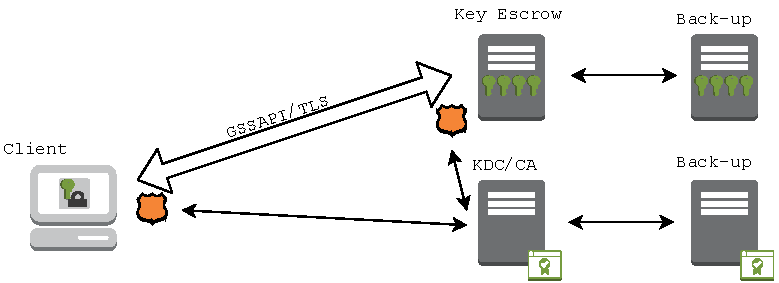
\includegraphics[scale=0.7]{figures/EscrowModel.pdf}
    \caption{Escrow model}
    \label{fig_escrowmodel}
\end{figure}
Unfortunately, this is not enough to have the communication secure.
This server has to have its identity verified, and the client has to authenticate to this server too.
The increasing amount of keys implicates a need for Certification Authority server (CA) or a Key Distribution Center (KDC) to manage all of them.

Only with the infrastructure in place and keys produced, the server can verify if the client is permitted to get their key, and the client is able to identify a trusted server.
This is a fully stateful process.

The complexity of this system increases the attack surface and for such complex system it would be unimaginable not to have backups.
The Escrow server may store lots of keys from lots of different places, users and services.



\section{Tang Server}\label{tang}

With key escrow, a third party gets copies of a cryptographic key.
People might not be comfortable with any third party having this ability and that “technical” problems vex the key escrow solution.
Tang's key recovery, on the other hand, lets us just “backup” and restore cryptographic keys anonymously and without any third party possesing our key.

Tang is a very lightweight network service using systemd's socket activation as described in section \ref{socket_activation}.
Its purpose is to provide anonymous key recovery to clients over the network.
This key recovery can be used with a help of the Tang's client descibed in subsection \ref{clevis} Clevis client to unlock data storages with LUKS encryption.
The Tang server is an open source project implemented in C programming language.

We can see on Figure \ref{fig_tangmodel} that the Tang model is very similar to the escrow seen on Figure \ref{fig_escrowmodel} but with some things missing.
\begin{figure}[h]
    \centering
    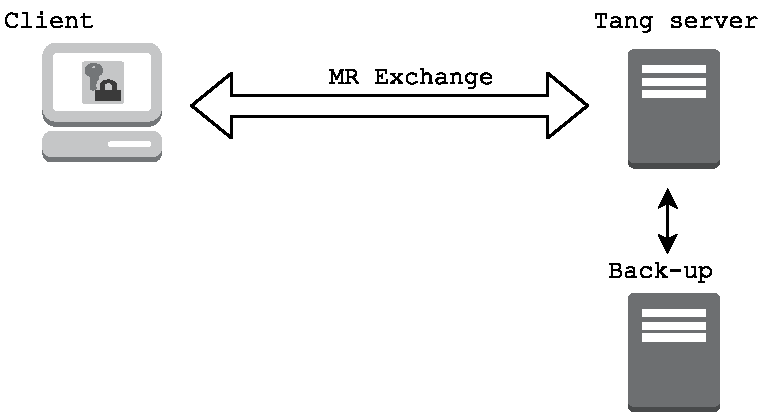
\includegraphics[scale=0.7]{figures/TangModel.pdf}
    \caption{Tang model}
    \label{fig_tangmodel}
\end{figure}
In fact, there is no longer need for TLS channel to secure communication between the client and the server,
 and that is because Tang implements the McCallum-Relyea exchange as described below.

Tang server advertises asymmetric keys on the network and a client is able to get the list of these signing keys by HTTP (Hypertext Transfer Protocol) GET request.
All tang communication is performed using the HTTP protocol with the message body in JWK (JSON Web Key) format defined by RFC 7517 \cite{RFC7517}.
Getting advertised keys is the first step of the McCallum-Relyea exchange protocol summed up in table \ref{mrexchange}.
\begin{table}[h]
\centering
\label{mrexchange}
\begin{tabular}{c|c|c|c}
\hline
\multicolumn{2}{c|}{Provisioning} & \multicolumn{2}{c}{Recovery} \\ \hline
client's side & server's side & client's side & server's side \\ \hline
 & $ S \epsilon _{bindingR} [1, p-1]$ & $E \epsilon _{R} [1, p-1]$ &  \\
 & $s = g * S$ &$ x = c + g * E$ &  \\
\multicolumn{2}{c|} {$\leftarrow$  s} & \multicolumn{2}{c} {x $\rightarrow$}  \\
$C \epsilon _{R} [1, p-1]$ &  &  & $y = z * S$\\
$e = g * C $&  & \multicolumn{2}{c} {$\leftarrow$ y} \\
$k = g * S * C = s * C$ &  & $k = y - s * E$&  \\
Discard: K, C &  &  &  \\
Retain s, c &  &  &  \\ \hline
\multicolumn{4}{c}{*capital is private key; g stands for generate}
\end{tabular}
\caption{McCallum-Relyea exchange protocol}
\end{table}
This protocol has two phases, provisioning and recovery.

\paragraph{Provisioning}
The server key pair generation is represented by equation \ref{servergen}, capital is private key; lowercase is public key; g stands for generate.
\begin{equation}\label{servergen}
    s = g * S
\end{equation}
After the server generates key pair, it is advertising the public part of it.
The client then selects one of the Tang server's exchange keys (we will call it {\it sJWK}; identified by the use of {\it deriveKey} in the {\it sJWK}'s {\it key\_ops} attribute).
The lowercase “s” stands for server's public key and JWK is format of the message.
The client then generates a new (random) JWK ({\it cJWK}; c stands for client's key pair).
\begin{equation}\label{clientgen}
    c = g * C
\end{equation}
The client performs its half of a standard ECDH exchange producing {\it kJWK} -- see equation \ref{kJWK_gen}, which it uses to encrypt the data.
Afterwards, it must discard the {\it kJWK} and the private key from {\it cJWK}.
\begin{equation}\label{kJWK_gen}
    k = s * C
\end{equation}
The client has to store {\it cJWK} for later use in the recovery step.
Generally speaking, the client may also store other data, such as the URL of the Tang server or the trusted advertisement signing keys called also binding keys.



\paragraph{Recovery}
Mathematically capital letter is private key; g stands for generate.
When the client wants to access the encrypted data, it must be able to recover encryption key.
To recover {\it kJWK} after discarding it, the client generates a third ephemeral key ({\it eJWK}) as the equation \ref{eqn_ephemeral} represent.
This key is used to hide the client's public key and the binding key.
\begin{equation}\label{eqn_ephemeral}
    e = g * E
\end{equation}
The ephemeral key is generated for each execution of a key establishment process.
Using {\it eJWK}, the client performs elliptic curve group addition of {\it eJWK} and {\it cJWK}, producing {\it xJWK} represented in the equation \ref{eqn_ecga}.
The client {\it POST}s {\it xJWK} to the server.
\begin{equation}\label{eqn_ecga}
    x = c + e
\end{equation}
The server then performs its half of the ECDH key exchange using {\it xJWK} and {\it sJWK}, producing {\it yJWK} reflected in the equation \ref{eqn_response}. The server returns {\it yJWK} to the client.
\begin{equation}\label{eqn_response}
    y = x * S
\end{equation}
The client then performs half of an ECDH key exchange between {\it eJWK} and {\it sJWK}, producing {\it zJWK} as the equation \ref{eqn_get} shows.
\begin{equation}\label{eqn_get}
    z = s * E
\end{equation}
Subtracting {\it zJWK} from {\it yJWK} produces {\it dJWK} shown in the equation \ref{eqn_extract}.
\begin{equation}\label{eqn_extract}
    k = y - z
\end{equation}
Finally, the client has calculated the key value.
So the Tang server never knows the value of the key and literally nothing about its clients.



\subsection{Security}

As shown in table \ref{compare}, Tang compared to Escrow is stateless and doesn't require TLS or authentication.
Tang also has limited knowledge.
Unlike escrows, where the server has knowledge of every key used, Tang never sees any client keys.
Tang never gains any identifying information from the client.

\begin{table}[h]
\centering
\label{compare}
\begin{tabular}{@{}lll@{}}
\toprule
               & Escrow   & Tang                         \\ \midrule
Stateless      & No       & Yes                          \\
SSL/TLS        & Required & Optional                     \\
X.509          & Required & Optional                     \\
Authentication & Required & Optional                     \\
Anonymous      & No       & Yes                          \\ \bottomrule
\end{tabular}
\caption{Comparing Escrow and Tang}
\end{table}

Thanks to McCallum-Relyea exchange protocol summed up in the table \ref{mrexchange} Tang is resistant to the man in the middle attack.
In case of the eavesdroppers, they see the client send {\it xJWK} and receive {\it yJWK}.
Since these packets are blinded by {\it eJWK}, only the party that can un-blind these values is the client itself (since only it has {\it eJWK}'s private key).
Thus, the attack fails.

It is of utmost importance that the client protects {\it cJWK} and the Tang server must protect the private key for {\it sJWK}.



\subsection{Building Tang}

Tang is originally packaged for Fedora operating system version 23 and later but we can of course build it from source.
It relies on few other software libraries listed in section \ref{dependencies}.

The steps to build the Tang from sources include downloading the source from project's GitHub or cloning~it.
Make sure all required dependencies are installed and then run:
\begin{lstlisting}[columns=fixed,basicstyle=\ttfamily\footnotesize,tabsize=4,backgroundcolor=\color{yellow!10}]
$ autoreconf -if
$ ./configure --prefix=/usr
$ make
# make install
\end{lstlisting}
Optionally tests can be run with:
\begin{lstlisting}[columns=fixed,basicstyle=\ttfamily\footnotesize,tabsize=4,backgroundcolor=\color{yellow!10}]
$ make check
\end{lstlisting}



\subsection{Server Enablement}

Enabling a Tang server is a two-step process.
First step is to enable the Tang services.
Start the key update service which is watching the database directory using systemd:
\begin{lstlisting}[columns=fixed,basicstyle=\ttfamily\footnotesize,tabsize=4,backgroundcolor=\color{yellow!10}]
# systemctl enable tangd-update.path --now
\end{lstlisting}
Enable service using systemd socket activation:
\begin{lstlisting}[columns=fixed,basicstyle=\ttfamily\footnotesize,tabsize=4,backgroundcolor=\color{yellow!10}]
# systemctl enable tangd.socket --now
\end{lstlisting}
After this, systemd will handle the sockets and the Tang's key rotation procedure.

Second, generate a signing key using dependency tool jose and store it in a default directory expected by tang:
\begin{lstlisting}[columns=fixed,basicstyle=\ttfamily\footnotesize,tabsize=4,backgroundcolor=\color{yellow!10}]
# jose gen -t '{"alg":"ES256"}' -o /var/db/tang/sig.jwk
\end{lstlisting}
Do not forget to generate an exchange key:
\begin{lstlisting}[columns=fixed,basicstyle=\ttfamily\footnotesize,tabsize=4,backgroundcolor=\color{yellow!10}]
# jose gen -t '{"kty":"EC","crv":"P-256","key_ops":["deriveKey"]}' \
        -o /var/db/tang/exc.jwk
\end{lstlisting}
These commands results into change in the Tang's database directory now containing the {\tt sig.jwk} and the {\tt exc.jwk}.
The {\tt tangd-update.path} service will trigger regeneration of the cache, stored in {\tt /var/cache/tang/} directory, using {\tt /usr/libexec/tangd-update} script.

Now we are up and running.
The server is ready to send an advertisement on client's demand or even using curl:
\begin{lstlisting}[columns=fixed,basicstyle=\ttfamily\footnotesize,tabsize=4,backgroundcolor=\color{yellow!10}]
curl -f http://tang.local/adv
\end{lstlisting}
Tang now advertises its {\tt exc.jwk} key signed using the {\tt sig.jwk}.

\subsection{Clevis Client}\label{clevis}

Clevis provides a pluggable key management framework for automated decryption and has full support for Tang.
It can handle automated unlocking of LUKS volumes.
Clevis lets us encrypt data with a simple command:
\begin{lstlisting}[columns=fixed,basicstyle=\ttfamily\footnotesize,tabsize=4,backgroundcolor=\color{yellow!10}]
$ clevis encrypt PIN CONFIG < PLAINTEXT > CIPHERTEXT.jwe
\end{lstlisting}
In clevis terminology, a {\it PIN} is a plugin which implements automated decryption.
We simply pass the name of the supported pin here.
Besides {\tt Tang} {\it PIN} clevis also supports a {\it PIN} for performing escrow using {\tt HTTP} or an {\tt SSS} {\it PIN} to provide a way to mix pins together to provide sophisticated unlocking policies by using an algorithm called Shamir Secret Sharing (SSS).%miso

Second, {\it CONFIG} is a JSON object which will be passed directly to the {\it PIN}.
It contains all the necessary configuration to perform encryption and setup automated decryption.


\paragraph{PIN: Tang} -- Here is an example of how to use Clevis with Tang:
\begin{lstlisting}[columns=fixed,basicstyle=\ttfamily\footnotesize,tabsize=4,backgroundcolor=\color{yellow!10}]
$ echo hi | clevis encrypt tang '{"url": "http://tang.local"}' > hi.jwe
The advertisement contains the following signing keys:

Apb39FO1vey9FyUe_fEd8lVDABs

Do you wish to trust these keys? [ynYN] y
$ clevis decrypt tang '{"url": "http://tang.local"}' < hi.jwe
hi
\end{lstlisting}
In this example, we encrypt the message “hi” using the {\tt Tang} {\it PIN}.
The only parameter needed in this case is the URL of the Tang server.
During the encryption process, the {\tt Tang} {\it PIN} requests the key advertisement from the server and asks us to trust the keys.
This works similarly to SSH.

Alternatively, we can manually load the advertisement using the adv parameter.
This parameter takes either a string referencing the file where the advertisement is stored, or the JSON contents of the advertisement itself.
When the advertisement is specified manually like this, Clevis presumes that the advertisement is trusted.



\subsection{Binding LUKS Volumes with Clevis}\label{dracut}
Tang's main purpose is to enable early boot decryption of the {\it LUKS} volumes and clevis is the client solution for it.
Clevis can be used to bind a {\it LUKS} volume using a {\it PIN} so that it can be automatically unlocked.

Clevis automatically generates a new, cryptographically strong key using the Tang's advertisement.
This key is added to {\it LUKS} as an additional passphrase.
Clevis then encrypt this key using Tang's advertisement, and store the output JWE (JSON Web Encryption) inside the {\it LUKS} header using {\it LUKSMeta} library.
Here is an example where we bind {\tt /dev/vda2} using the Tang ping:
\begin{lstlisting}[columns=fixed,basicstyle=\ttfamily\footnotesize,tabsize=4,backgroundcolor=\color{yellow!10}]
# clevis bind-luks /dev/sda1 tang '{"url": "http://tang.local"}'
The advertisement is signed with the following keys:
        kWwirxc5PhkFIH0yE28nc-EvjDY

Do you wish to trust the advertisement? [yN] y
Enter existing LUKS password:
\end{lstlisting}

Upon successful completion of this binding process, the disk can be unlocked using one of the unlockers described below.



\paragraph{Dracut}\label{dracut}Install it to Fedora using:
\begin{lstlisting}[columns=fixed,basicstyle=\ttfamily\footnotesize,tabsize=4,backgroundcolor=\color{yellow!10}]
# dnf install clevis-dracut
\end{lstlisting}

The Dracut unlocker attempts to automatically unlock volumes during early boot.
This permits the automated root volume encryption.
To unlock Fedora, initramfs must be rebuilt after installing Clevis using:

\begin{lstlisting}[columns=fixed,basicstyle=\ttfamily\footnotesize,tabsize=4,backgroundcolor=\color{yellow!10}]
# dracut -f
\end{lstlisting}
Upon reboot, we will be prompted to unlock the volume using a password.
In the background, Clevis will attempt to unlock the volume automatically.
If it succeeds, the password prompt will be canceled and boot will continue.



\paragraph{UDisks2}\label{udisk2}
After installation, UDisks2 unlocker runs in a Fedora desktop session.
There is no need to manually enable it; just install the Clevis UDisks2 unlocker and restart desktop session.
\begin{lstlisting}[columns=fixed,basicstyle=\ttfamily\footnotesize,tabsize=4,backgroundcolor=\color{yellow!10}]
# dnf install clevis-udisks2
\end{lstlisting}
The unlocker should be started automatically.
This unlocker works almost exactly the same as the Dracut unlocker.
If we insert a removable storage device that has been bound with Clevis, it will attempt to unlock it automatically in parallel with a desktop password prompt.
If automatic unlocking succeeds, the password prompt will be dissmissed without user intervention.

  \chapter{Software portability}\label{porting}

Ideally, any software would be usable on any operating system, platform, and any processor architecture.
Existence of term "porting", derived from the Latin portāre which means "to~carry", proves that this ideal situation does not occurs that often, and acctual process of "carrying" software to system with different environment is most probably required.
Porting is not documented process required to adapt software designed for specific platform to another platform.
Porting is also used to describe procces of converting computer games to became platform independent\cite{wiki_porting}.

Software porting procces might be hard to distinguish with building software.
The reason might be that in many cases building software on desired platform is enough, when software application does not work "out of the box".
This kind of behavior, an application that works immediately after or even without any special installation and without need for any configuration or modification, is ideal.
It often happens when we copy application from one computer to another, not realizing that they have processors with same instructions set and same or very similar operating system therefore envoroment.
But let us be realistic, it depends on many things, such as processor architecture to which was application written (compiled), quality of design, how application is meant to be deployed and of course application's source code.

Nowadays, the goal should be to develop software which is portable between preferred computer platforms (Linux, UNIX, Apple, Microsoft).
If software is considered as not portable, it could not have to mean immediately that it is not possible, just that time and resources spent porting already written software are almost comparable, or even significantly higher than writing software as a whole from scratch.
Effort spent porting some software product to work on desired platform must be little, such as copying already installed files to usb flash drive and run it on another computer.
This kind of approach might most probably fail, due to not present dependencies of third party libraries on destination computer.
Despite dominance of the x86 architecture there is usually a need to recompile software running, not only on different operating systems, to make sure we have all the dependencies present.

Number of significantly different central processor units (CPUs), and operating systems used on the desktop or server is much smaller than in the past.
However on embeded devices market there are still much more various architectures available including ARM\footnote{https://www.arm.com/products/processors} or MIPS\footnote{https://www.mips.com/products/classic/}.

To simplify portability, even on distinguished processors with distant instruction sets, modern compilers translate source code to a machine-independent intermediate code.
But still, in the embedded system market, where OpenWrt belongs to, porting remains a significant issue \cite{porting_software}.



\section{OpenWrt system}\label{owrt}
OpenWrt is is perhaps the most widely known Linux distribution for embedded devices especially for wireless routers.
It was originally developed in January 2004 for the Linksys WRT54G with buildroot from the uClibc project.
Now it supports many more models of routers.
OpenWrt is a registered trademark which is held by the Software in the Public Interest (SPI) in the name of the OpenWrt project.

Installing OpenWrt system means replacing our router’s built-in firmware with the Linux system which provides a fully writable filesystem with package management.
This means that we are not bound to applications provided by the vendor.
Router (the embedded device) with this distribution can be used for anything that an embedded Linux system can be used for, from using its SSH Server for SSH Tunneling, to running lightweight server software (e.g. IRC server) on it.
In fact it allows us to customize the device through the use of packages to suit any application. \cite{openwrt}



\subsection{OpenWrt and LEDE}

The LEDE Project (“Linux Embedded Development Environment”) is a Linux operating system emerged from the OpenWrt project.
Its announcement was sent on 3th May 2016 by Jo-Philipp Wich to both the OpenWrt development list and the new LEDE development list\footnote{https://lwn.net/Articles/686180/}.
It describes LEDE as "a reboot of the OpenWrt community" and as "a spin-off of the OpenWrt project" seeking to create an embedded-Linux development community "with a strong focus on transparency, collaboration and decentralisation"\footnote{https://www.phoronix.com/scan.php?page=news\_item\&px=OpenWRT-Forked-As-LEDE}.

The rationale given for the reboot was that OpenWrt suffered from longstanding issues that could not be fixed from within—namely, regarding internal processes and policies.
For instance, the announcement said, the number of developers is at an all-time low, but there is no process for on-boarding new developers and, it seems, no process for granting commit access to new developers.

At the moment latest release of OpenWrt 15.05.1 (code-named "Chaos Calmer") released in March 2016.
LEDE developers continued to work separately on their upstream release and they delivered LEDE "Reboot" with version 17.01.0 on February 22nd 2017.

The remerge proposal vote was passed by LEDE developers in June 2017\footnote{http://lists.infradead.org/pipermail/lede-adm/2017-June/000552.html}.
After long and sometimes slowly moving discussions about the specifics of the re-merge, with multiple similar proposals but little subsequent action, formally announced on LEDE forum in January 2018\footnote{https://forum.lede-project.org/t/announcing-the-openwrt-lede-merge/10217}.
OpenWrt and LEDE projects agreed upon their unification under the OpenWrt name.
After merge OpenWrt upstream repository started to show signs of life.

Today (April 2018) the stable LEDE 17.01.4 "Reboot" release of OpenWrt released in October 2017 using Linux kernel version 4.4.92 runs on many routers \cite{lede_release}.



\subsection{Why use OpenWrt}

Custom router firmware may be more stable than our hardware’s default firmware from the vendor.
Not even that but probably more secure with regullar security updates.
Besides OpenWrt there are other open source Linux based firmwares available such as Tomato or DD-WRT.

In the past OpenWrt has supported only CLI (command line interface) configuration therefore it was best match for software developers, network admins, or advanced users.
User not acquainted with Linux or even not comfortable with CLI found the OpenWrt platform hard to use and they turned to other solutions available.

The Tomato firmware is the best match for unexperienced users providing rich GUI and many features specifically live "visual" traffic monitoring, allowing easy visibility on inbound/outbound traffic in real-time.
Big disadvantage of the Tomato is that list of supported devices is quite poor.

DD-WRT on the other hand is compatible with more routers than any other third party firmware.
Compared to Tomato, DD-WRT is reported to have more bugs and less intuitive GUI.
The DD-WRT was known as the most feature rich firmware until OpenWrt came along.

OpenWrt turns our router in a fully capable GNU/Linux computer, not just a network "magic" box.
Last years the OpenWrt platform has come a long way in making itself more accessible to all user levels.
It has an Luci\footnote{https://github.com/openwrt/luci} Web UI(user interface) now.
Users less experienced with Linux can easily set up their network using Luci.
OpenWrt is capable of running lightweight services like an IRC bouncer or samba/ftp file sharing (some routers has USB ports able to power HDD) or even run software build on our own\cite{vpnpick}.

The goal of this thesis would be to port a lightweight Tang daemon described in the section \ref{tang} Tang to OpenWrt system.
Tang server will help us unlock our encrypted volumes while on safe home or office network without need for extra PC running it but having it on our tiny OpenWrt "server".
With Tang we do not have to care about typing passphrases over and over to unlock LUKS drives in safe enviroment.



\section{OpenWrt's toolchain}

Embeded devices are not meant for building on them because they does not have enough memory nor computation resorces as ordinary personal computers do(see Table \ref{routerspec}).
Building on such device would be time consuming and may result to overheating, which could cause hardware to fail.
For this particular reason package building is done with cross-compiler.
Compilation is done by set of tools called toolchain and it consists of:
\begin{itemize}
    \item compiler
    \item linker
    \item a C standard library
\end{itemize}
For porting to "target" system (OpenWrt) this toolchain has to be generated on "host" system.
The toolchain can be achieved in many different ways.
The easiest way is undoubtedly to find a .rpm (.deb or any distribution specific available) package and have it installed on our "host" system.
If a binary package with desired toolchain is not available for our system or is not available at all, there might be need to compile a custom toolchain from scratch.\footnote{tools like crosstool-ng (https://github.com/crosstool-ng/crosstool-ng) may help}

In case of OpenWrt we have available a set of Makefiles and patches called buildroot which is capable of generating toolchain.



\subsection{Compiler}

In a nutshell compilers translate the high level programming language source code into lower level language such as machine understandable assembler instructions.
To do so compiler is performing many operations starting with preprocessing.

Preprocessing supports macro substitution and conditional compilation.
Typically the preprocessing phase occurs before syntactic or semantic analysis.
However, some languages such as Scheme\footnote{https://www.scheme.com/tspl4/} support macro substitutions based on syntactic forms.

Lexical analysis, also known as lexing or tokenization, breaks the source code text into a sequence of small pieces called lexical tokens.
Lexical analyzer does the scanning (cutting the input text into tokens and assign them a category) and the evaluating (converting tokens into a processed value).
Common token categories may include:
\begin{itemize}
    \item keywords (bound to programming language)
    \item identifiers (can not be keyword)
    \item separators
    \item operators
    \item literals
    \item comments
\end{itemize}
The set of token categories varies in different programming languages.
The lexeme syntax is typically a regular language, so a finite state automaton constructed from a regular expression can be used to recognize it.

Syntax analysis typically builds a parse tree structure according to the rules of a formal grammar which define the language's syntax.
The parse tree is often analyzed, augmented, and transformed by later phases in the compiler.

Semantic analysis checks parse tree and does type checking, object binding and definite assignment.
Output of semantic analysis is the symbol table or it results into rejecting incorrect programs or issuing warnings.

Code optimization, such as dead code elimination, inline expansion, constant propagation, loop transformation and even automatic parallelization, is done after analysis and it is independent on the CPU architecture.

Code generation is CPU dependent and does the transformation of intermediate language into the target machine language.
This involves resource and storage decisions, such as deciding which variables to fit into registers and memory and generating machine instructions along with their associated addressing modes.

Cross-compiler is programming tool capable of creating executable file that is supposed to run on a "target" architecture, in a similar or completely different enviroment, while working on a different "host" architecture.
It can also create object files used by linker.
Reason for using cross-compiling might be to separate the build environment from target environment as well.
OpenWrt toolchain uses gcc compiler, and it is one of the most important parts of toolchain\cite{compiler}.



\subsection{Linker}

With linker we are able to link compile's object files into single executable, library or object file.
Linker can do static linking and dynamic linking.

Static linking is the result of the linker copying all library routines used in the program into the executable image.
This may require more disk space and memory than dynamic linking, but is more portable, since it does not require the presence of the library on the system where it runs.
Static linking also prevents "DLL Hell", since each program includes exactly the versions of library routines that it requires, with no conflict with other programs. In addition, a program using just a few routines from a library does not require the entire library to be installed.

Dynamic linking is the process of postponing the resolving of some undefined symbols until a program is run.
That means that the executable code still contains undefined symbols, plus a list of objects or libraries that will provide definitions for these.
Loading the program will load these objects/libraries as well, and perform a final linking.
Dynamic linking needs no linker.

Advantage of dynamic linking is that often-used libraries (for example the standard system libraries) need to be stored in only one location, not duplicated in every single binary.
If a bug in a library function is corrected by replacing the library, all programs using it dynamically will benefit from the correction after restarting them.
Programs that included this function by static linking would have to be re-linked first.

Disadvantage known on the Windows platform as "DLL Hell", an incompatible updated library will break executables that depended on the behavior of the previous version of the library if the newer version is not properly backward compatible\cite{compiler}.



\subsection{C standard library}

Most common C standard libraries are: GNU Libc, uClibc musl-libc, or dietlibc.
They provide macros, type definitions and functions for tasks such as input/output processing (<stdio.h>), memory management (<stdlib.h), string handling (<string.h>), mathematical computations (<math.h>) and many more\footnote{https://en.wikipedia.org/wiki/C\_standard\_library\#Header\_files}.
The OpenWrt's cross-compilation toolchain uses musl-libc \cite{c_library}.



\section{OpenWrt's buildroot}

OpenWrt's buildroot is a build system capable of generating toolchain, and also a root filesystem (also called sysroot), enviroment tightly bound to target.
Build system can be configured for any device that is supported by OpenWrt.

The root filesystem in general is a mere copy of the file system of target's platform.
In many cases just having the folders /usr and /lib would be sufficient, therefore we do not need to copy nor create the entire target file system on our host .

It is a good idea to store all these things, the toolchain and the root filesystem in a single place.
With using OpenWrt's buildroot we will have this covered.
Be tidy and pedantic, because cross-compiling can easily become a painful mess!



\subsection{Buildroot prerequisites}

Let us demonstrate what are minimum requirements of space and size of RAM (Random Access Memory) for building packages for Openwrt using its buildroot.
For generating an installable OpenWrt firmware image file with a size of e.g. 8MB, we will need at least:
\begin{itemize}
\item ca. 200 MB for OpenWrt build system
\item ca. 300 MB for OpenWrt build system with OpenWrt Feeds
\item ca. 2.1 GB for source packages downloaded during build from the Feeds
\item ca. 3-4 GB to build (i.e. cross-compile) OpenWrt and generate the firmware file
\item ca. 1-4 GB of RAM to build Openwrt.(build x86's img need 4GB RAM)
\end{itemize}

These are specifications of embedded device TL-WR842Nv3 a regular wireless router manufactured by TP-LINK which was used to test all packages related to Tang server porting effort:

\begin{table}[h]
\centering
\label{routerspec}
\begin{tabular}{c|c}
\hline
Model           &   TL-WR842N(EU)                   \\ \hline
Version         &   v3                              \\ \hline
Architecture:   &   MIPS 24Kc                       \\ \hline
Manufacturer:   &   Qualcomm Atheros                \\ \hline
Bootloader:     &   U-Boot                          \\ \hline
System-On-Chip: &   Qualcomm Atheros QCA9531-BL3A   \\ \hline
CPU Speed:      &   650 MHz                         \\ \hline
Flash chip:     &   Winbond 25Q128CS16              \\ \hline
Flash size:     &   16 MiB                          \\ \hline
RAM chip:       &   Zentel A3R12E40CBF-8E           \\ \hline
RAM size:       &   64 MiB                          \\ \hline
Wireless:       &   Qualcomm Atheros QCA9531        \\ \hline
Antenae(s):     &   2 non-removable                 \\ \hline
Ethernet:       &   4 LAN, 1 WAN 10/100             \\ \hline
USB:            &   1 x 2.0                         \\ \hline
Serial:         &   No                              \\ \hline
\end{tabular}
\caption{TL-WR842Nv3 specifications}
\end{table}

The actual sum of space required only for buildroot to work correctly which is about 6.4 GB.
Comparation to available storage space on wireless router should demonstrate why is building for embedded devices done with cross-compiling.
The another reasons, not to just compare internal storage which might be extended\footnote{https://wiki.openwrt.org/doc/howto/extroot} are device's minimalistic RAM size and lower computation capability of the CPU.



\section{Preparing the host enviroment}

To start with cross-compilation on the host system we need to set up an enviroment for it.
As the OpenWrt buildroot is set of scripts it has runtime dependencies.
We need to install these dependencies first.
To install buildroot dependencies on Fedora 27 system run:
\begin{lstlisting}[columns=fixed,basicstyle=\ttfamily\footnotesize,tabsize=4,backgroundcolor=\color{yellow!10}]
# dnf install binutils bzip2 gcc gcc-c++ \
gawk gettext git-core flex ncurses-devel ncurses-compat-libs \
zlib-devel zlib-static make patch perl-ExtUtils-MakeMaker \
perl-Thread-Queue  glibc glibc-devel glibc-static quilt sed \
sdcc intltool sharutils bison wget unzip openssl-devel
\end{lstlisting}
Some feeds (the OpenWrt packages) might be not available over git but only via other versioning tools like svn (subversion) or mercurial.
If we want to obtain their source-code, we need to install svn and mercurial as well:
\begin{lstlisting}[columns=fixed,basicstyle=\ttfamily\footnotesize,tabsize=4,backgroundcolor=\color{yellow!10}]
# dnf install subversion mercurial
\end{lstlisting}
Please note that these commands have to be run by user with root privileges.



\subsection{Getting buildroot}

OpenWrt system has available an SDK(Software development kit) buildroots for every released version of OpenWrt system.
It is good to consider using OpenWrt's SDK in order to build software application to only one specific release of target system.
For example when we are using "stable" release of OpenWrt 15.05.1 with codename "Chaos Calmer" on TL-WR842N(EU) device, we should probably end up in in "Supplementary Files" section of the OpenWrt archives
\footnote{https://archive.openwrt.org/chaos\_calmer/15.05.1/ar71xx/generic/} looking for the SDK.
While porting an upstream projets (such as Tang) for latest target release a bleeding edge buildroot would be the best solution.

If we have host platform which aims to be on the bleeding edge of open-source technologies, such as OS Fedora, we will probably encounter issues with dependencies.
These issues are apearing because an older version of the dependencies are required for this old SDK to work and might be not available for our host platform anymore.
In this case we would have to install or even build older version of required packages.

We will work with bleeding edge (trunk version) buildroot and build for latest LEDE 17.01.4 release.
To clone upstream buildroot run command:
\begin{lstlisting}[columns=fixed,basicstyle=\ttfamily\footnotesize,tabsize=4,backgroundcolor=\color{yellow!10}]
$ git clone https://github.com/openwrt/openwrt.git
\end{lstlisting}

\section{Working with buildroot}\label{working-with-buildroot}

Working with Openwrt's buildroot requires some basic knowledge of the git version control system\footnote{https://git-scm.com/docs/gittutorial} and processes of upstream project development using GitHub\footnote{https://guides.github.com/introduction/flow/}.
Short description how to fork and set up repository can be found on appendix \ref{set_repo} Setting up the repository.
All work related to this thesis has been done using GitHub account Tiboris\footnote{https://github.com/Tiboris/} therefore following command to get our fork of buildroot would be:
\begin{lstlisting}[columns=fixed,basicstyle=\ttfamily\footnotesize,tabsize=4,backgroundcolor=\color{yellow!10}]
$ git clone https://github.com/Tiboris/openwrt.git ~/buildroot-openwrt
\end{lstlisting}

After we have enviroment ready to be worked on (all needed dependencies installed and fork of our buildroot downloaded on host system) let us just follow these simple 4 rules to not break our enviroment in any way.
\begin{enumerate}
    \item Do everything in buildroot as non-root user!
    \item Issue all OpenWrt build system commands in the <buildroot> directory, \\e.g. $\sim$/buildroot-openwrt/
    \item Do not build in a directory that has spaces in its full path.
    \item Change ownership of the directory where we downloaded \\the OpenWrt to other than root user
\end{enumerate}
Having these in mind will definitely make our work easier.



\subsection{Setting feeds}

In OpenWrt, a "feed" is a collection of packages which share a common location.
Feeds may reside on a remote server, in a version control system, on the local filesystem, or in any other location addressable by a single name (path/URL) over a protocol with a supported feed method.
It is the most important step to do before starting cross-compilation.
As the listing \ref{default_feeds} Content of feeds.conf.default shows a list of usable feeds is configured from the feeds.conf file or feeds.conf.default when feeds.conf does not exist.

\begin{lstlisting}[columns=fixed,basicstyle=\ttfamily\footnotesize,tabsize=4,label=default_feeds,caption=Content of feeds.conf.default]
    src-git packages https://git.openwrt.org/feed/packages.git
    src-git luci https://git.openwrt.org/project/luci.git
    src-git routing https://git.openwrt.org/feed/routing.git
    src-git telephony https://git.openwrt.org/feed/telephony.git
    #src-git video https://github.com/openwrt/video.git
    #src-git targets https://github.com/openwrt/targets.git
    #src-git management https://github.com/openwrt-management/packages.git
    #src-git oldpackages http://git.openwrt.org/packages.git
    #src-link custom /usr/src/openwrt/custom-feed
\end{lstlisting}

The new custom OpenWrt packages are located in packages feed (see the first line of the \ref{default_feeds} Content of feeds.conf.default listing).
To work with our own fork of the packages we can simply change the line to point to our fork repository.
Feeds can point to special branch of our choice:
\begin{lstlisting}[columns=fixed,basicstyle=\ttfamily\footnotesize,tabsize=4,backgroundcolor=\color{yellow!10}]
src-git packages https://github.com/Tiboris/packages-OpenWrt.git;new_packages
\end{lstlisting}
or commit hash in repository:
\begin{lstlisting}[columns=fixed,basicstyle=\ttfamily\footnotesize,tabsize=4,backgroundcolor=\color{yellow!10}]
src-git packages https://github.com/Tiboris/packages-OpenWrt.git^dbdfc99
\end{lstlisting}
Changing this feed to will reduce effort spending on getting all new dependencies to the buildroot's feeds/packages directory.

The feeds are "managed" with the script available in builroot's scripts directory, {\it feeds}.
To download feeds run this script with command {\it update} and option {\it -a}.
Remember to invoke it from the buildroot directory($\sim$/buildroot-openwrt).
\begin{lstlisting}[columns=fixed,basicstyle=\ttfamily\footnotesize,tabsize=4,backgroundcolor=\color{yellow!10}]
$ ./scripts/feeds update -a
\end{lstlisting}

To make any feed available for build we shall "install" it using the same feeds script:
\begin{lstlisting}[columns=fixed,basicstyle=\ttfamily\footnotesize,tabsize=4,backgroundcolor=\color{yellow!10}]
$ ./scripts/feeds install <PACKAGENAME>
\end{lstlisting}
or we can use option {\it -a} instead of the {\it <PACKAGENAME>} and make all of the feeds available for build.

If for some unknown reason the issued update of packages does not seems to show all the updates it might be helpful to clean the buildroot's {\it tmp/} directory\cite{feeds}.
\begin{lstlisting}[columns=fixed,basicstyle=\ttfamily\footnotesize,tabsize=4,backgroundcolor=\color{yellow!10}]
$ rm -rf tmp/
\end{lstlisting}

\subsection{The menuconfig}

For OpenWrt it has been the intention from the beginning, with the development of menuconfig, to create a simple, yet powerful, environment for the configuration of individual builds.
Working with menuconfig is very intuitive and the tool is more or less self-explanatory.
Even the most specialized configuration requirements can be met by using it.
Depending on the particular target platform, package requirements and kernel module needs, the standard configuration process will include modifying:
\begin{itemize}
    \item Target system
    \item Package selection
    \item Build system settings
    \item Kernel modules
\end{itemize}

Start the menuconfig interface shown on Figure \ref{fig_menuconfig} menuconfig by issuing the following command:
\begin{lstlisting}[columns=fixed,basicstyle=\ttfamily\footnotesize,tabsize=4,backgroundcolor=\color{yellow!10}]
$ make menuconfig
\end{lstlisting}
The make menuconfig will collect package info first.
Afterwards the following window will appear in our terminal and there we can start configuring the image using menuconfig:
\begin{figure}[h]
    \centering
    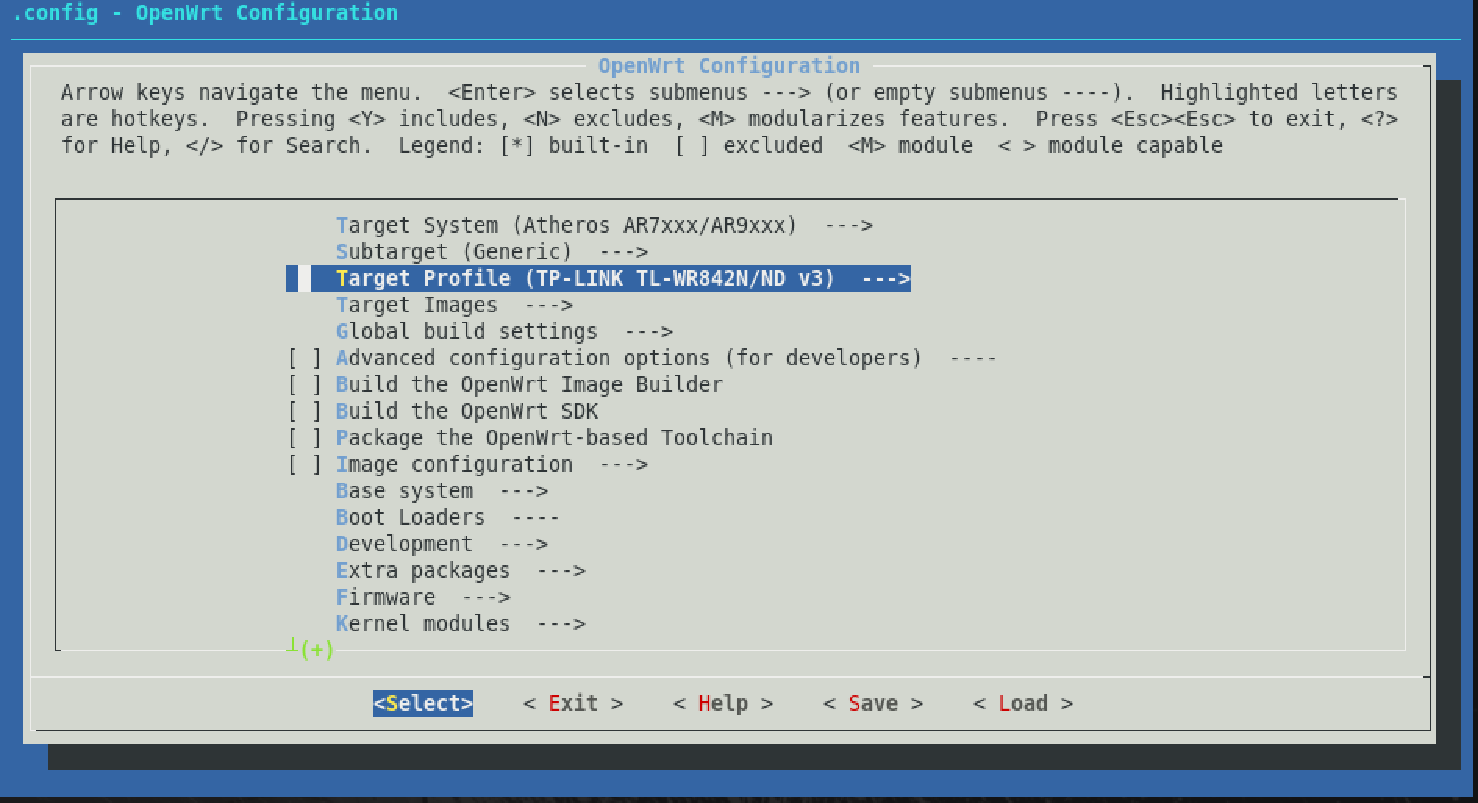
\includegraphics[scale=0.6]{figures/make_menuconfig.pdf}
    \caption{menuconfig}
    \label{fig_menuconfig}
\end{figure}

For configuring the image we have three options: y, m, n which are represented as follows:
\begin{itemize}
\item pressing y sets the <*> built-in label\\
This package will be compiled and included in the firmware image file.
\item pressing m sets the <M> package label\\
This package will be compiled, but not included in the firmware image file. (E.g. to be installed with opkg after flashing the firmware image file to the device.)
\item pressing n sets the < > excluded label\\
The source code will not be processed.
\end{itemize}
When we save our configuration, the file .config will be created in the buildroot directory according to desired configuration.

Target system is selected from the extensive list of supported platforms, with the numerous target profiles – ranging from specific devices to generic profiles, all depending on the particular device at hand.
In our case we should browse the "Target Profile" selection and find our targeted device (TP-LINK TL-WR842N/ND v3).

Package selection has the option of either 'selecting all package', which might be un-practical in certain situation, or relying on the default set of packages will be adequate or make an individual selection.
It is here needed to mention that some package combinations might break the build process, so it can take some experimentation before the expected result is reached.
Added to this, the OpenWrt developers are themselves only maintaining a smaller set of packages – which includes all default packages – but, the feeds-script makes it very simple to handle a locally maintained set of packages and integrate them in the build-process.

The final step before the process of compiling the intended image would be to exit the menuconfig tool – this also includes the option to save a specific configuration or load an already existing, and pre-configured, version.
Exit the UI, and choose to save the settings\cite{build_owrt}.



\subsection{Building single Packages}

When developing or packaging software for OpenWrt, it is convenient to be able to build only the package in question (e.g. with package cups):
\begin{lstlisting}[columns=fixed,basicstyle=\ttfamily\footnotesize,tabsize=4,backgroundcolor=\color{yellow!10}]
$ make package/cups/compile V=s
\end{lstlisting}
For a rebuild run:
\begin{lstlisting}[columns=fixed,basicstyle=\ttfamily\footnotesize,tabsize=4,backgroundcolor=\color{yellow!10}]
$ make package/cups/{clean,compile,install} V=s
\end{lstlisting}
It doesn't matter what feed the package is located in, this same syntax works for any installed package.

If for some reason the build fails, the easiest way to spot the error is to do:
\begin{lstlisting}[columns=fixed,basicstyle=\ttfamily\footnotesize,tabsize=4,backgroundcolor=\color{yellow!10}]
$ make V=s 2>&1 | tee build.log | grep -i error
\end{lstlisting}
Complete guide can be found on OpenWrt Wiki\footnote{https://wiki.openwrt.org/doc/howto/build}.

  \chapter{Porting the dependencies}\label{tangservice}

Programs don’t run in a vacuum but they interface with the outside world.
The view of this outside world differs from environment to environment.
Things like hostnames, system resources, and local conventions could be different.

When we start porting a code to a specific target platform, in our case OpenWrt, it is likely that we will face the first problem: satisfying missing dependencies.
This problem is easy to solve in principle, but can easily mess things up to a level we wouldn’t imagine.

If the code depends on some library that is NOT in the root filesystem, there’s no way out but to find them somewhere, somehow.
Dependencies can be satisfied in two ways: with static libraries or with shared libraries.
If we are lucky, we could find a binary package providing what we need (i.e. the library files and the header files), but most often we will have to cross-compile the source code on our own.
Either ways, we end up with one or more binary files and a bunch of header files.
Where to put them? Well, that depends.
There are a few different situations that can happen, but basically everything reduces to having dependencies in buildroot's root filesystem or in a different folder.

Having dependencies in a different folder could be an interesting solution to keep the libraries that we cross-compiled on our own separated from the other libraries (for example, the system libraries).
We can do that if we want but if we do, we must remember to provide to compiler and linker programs with the paths where header files and binary files can be found.
With static libraries, this information are only needed at compile and linking time, but if we are using shared libraries, this won’t suffice.
We must also specify where these libraries can be found at run time.

If we are satisfying the dependencies with shared libraries (.so files) having dependencies in root filesystem is probably the most common solution (and maybe, the best solution).
Remember that when everything will be up and running, these libraries must be installed somewhere in the file system of the target platform.
So there is a natural answer to the question above: install them in the target's root filesystem, for example in /usr/lib (the binary shared files) and /usr/include (the header files) or in any other path that allow the loader to find those libraries when the program executes.
Do not forget to install them in the file system of the actual target machine, in the same places, in order to make everything work as expected.
Please note that static libraries (‘.a’ files) does not need to be installed in the target file system since their code is embedded in the executable file when we cross-compile a program.
In case of OpenWrt we will use this approach.



\section{Find the depencies}

To port Tang to OpenWrt system we have have all its dependencies available and installed in buildroot.
First thing we should do is some digging and find out if dependencies for our software, we are about to port, are available for target's platform.
All packages available for OpenWrt can be found in its github repositories.
Let us remember Tang's dependencies first:

\begin{itemize}
\item http-parser
\item systemd's socket activation
\item José
    \begin{itemize}
    \item jansson
    \item openssl
    \item zlib
    \end{itemize}
\end{itemize}

After some digging we will find out that the OpenWrt system has already packages openssl, zlib, http-parser, and jansson.
Packages openssl and zlib are in versions already sufficient for Tang to get things work.

Package http-parser was little bit tricky.
At first try there is a chance that we will not find this package in OpenWrt's repository.
The reason might be that we will try to find a exactly "http-parser" string in OpenWrt's GitHub repository openwrt/openwrt only.
First of all, we must not forget that feeds of many packages are living in repository packages nested under openwrt organization.
Secondly after searching repository openwrt/packages for http-parser we will find out that it is named as libhttp-parser and in version 2.2.3.
This, let us say naming convention, is really common in Linux and could be predictable as the http-parser is in fact only a library.
One way or another compared to fedora packages it needs to be updated to latest version.

Jansson package was only available in version 2.7 which is too outdated for Tang's dependency José because it require at least jansson version 2.10.
We shall not forget that there is a need for updating jansson package for OpenWrt platform as well so we will do updates first.

Packages José, Tang and systemd are not listed in OpenWrt's packages.
Porting of the systemd would be huge effort but tang's requirements are minimal and we should be able to work with xinetd's socket activation.
Finally, as José and Tang are not listed in packages they will require to add them into package feeds to port Tang itself.

We will use fork of openwrt/packages repository placed outside of the buildroot package:
\begin{lstlisting}[columns=fixed,basicstyle=\ttfamily\footnotesize,tabsize=4,backgroundcolor=\color{yellow!10}]
$ git clone git@github.com:Tiboris/packages-OpenWrt.git
\end{lstlisting}



\section{Update outdated packages}

Finding that some of dependencies are already available on our desired target platform will definitelly make us satisfied.
We would agree that starting with something already built for OpenWrt is the best thing to do when we are approaching unknown platform.
In following subsections we will use all things we know from section \ref{working-with-buildroot} Working with buildroot.
Let us start with missing update of José's dependency, package jansson.


\subsection{Update jansson}\label{jansson}
Jansson is a C library for encoding, decoding and manipulating JSON data.
The latest release of the jansson is v2.11 released on 11th of February 2018\cite{jansson}.

However at the begining of the Tang porting efort started the latest release was v2.10.
To update mentioned OpenWrt available jansson package version v2.7 to 2.10 change to package's fork directory and create a new branch for changes:

\begin{lstlisting}[columns=fixed,basicstyle=\ttfamily\footnotesize,tabsize=4,backgroundcolor=\color{yellow!10}]
$ cd ~/packages-OpenWrt
$ git checkout -b jansson-update
\end{lstlisting}
In order to tell the OpenWrt buildroot how to build a program we need to create a special Makefile in the appropriate directory.
The appendix \ref{hello_mkfile} Example OpenWrt package's Makefile ilustrate its content.
We shall now find the jansson package Makefile in the repository using for example:
\begin{lstlisting}[columns=fixed,basicstyle=\ttfamily\footnotesize,tabsize=4,backgroundcolor=\color{yellow!10}]
$ git grep jansson | grep PKG_NAME
libs/jansson/Makefile:PKG_NAME:=jansson
\end{lstlisting}
The {\it PKG\_NAME} variable is one that identifies package for OpenWrt buildroot\cite{creating_pkgs}.
List of all available variables can be found on the OpenWrt wiki page\footnote{https://wiki.openwrt.org/doc/devel/packages}.
We can assume that the jansson library related files are located in libs/jansson directory of the packages repository.
Now we can now update Makefile.

We will open it with our preferred editor and find variable {\it PKG\_VERSION}.
Edit the old version number (in our case 2.7) to new version number (2.10).
This edit will result into changing the {\it PKG\_SOURCE} variable in Makefile.
Variables {\it PKG\_SOURCE} and {\it PKG\_SOURCE\_URL} are used to identify location of the archive with sources for specified version from where the sources would be downloaded.
After the downaload the OpenWrt buildroot checks the file integrity.
The {\it PKG\_HASH} and {\it PKG\_MD5SUM} variables serve this purpose.
As the new version of archive with sources will be downloaded we need to change {\it PKG\_HASH}/{\it PKG\_MD5SUM} variable as well.
For some reason upstream developers required the use of {\it PKG\_HASH} variable and the bz2 archive for the jansson package.
In general it would be sufficient to change only version and the appropriate {\it PKG\_HASH}/{\it PKG\_MD5SUM} variable.
We changed the filename extension for {\it PKG\_SOURCE} variable from ".tar.gz" to ".tar.bz2".
Now download the archive containing sources and get the archive hash using sha256sum:
\begin{lstlisting}[columns=fixed,basicstyle=\ttfamily\footnotesize,tabsize=4,backgroundcolor=\color{yellow!10}]
$ wget http://www.digip.org/jansson/releases/jansson-2.10.tar.bz2 -P /tmp
$ sha256sum /tmp/jansson-2.10.tar.bz2 | cut -d " " -f1
241125a55f739cd713808c4e0089986b8c3da746da8b384952912ad659fa2f5a
\end{lstlisting}
Last but not least commit the changes and push the changes into our fork.
\begin{lstlisting}[columns=fixed,basicstyle=\ttfamily\footnotesize,tabsize=4,backgroundcolor=\color{yellow!10}]
$ git commit -a
$ git push --set-upstream origin jansson-update
\end{lstlisting}

Before submitting the pull request we should try to build updated package first.
Let us remember that we have special branch set up for buildroot feeds.
We will use this branch to merge our newly created branch into it using:
\begin{lstlisting}[columns=fixed,basicstyle=\ttfamily\footnotesize,tabsize=4,backgroundcolor=\color{yellow!10}]
$ git checkout new_packages
$ git merge jansson-update
\end{lstlisting}
After successfull merge we have updated jansson package available in our custom feeds.
Trigger update with feeds script and make jansson available in menuconfig with:
\begin{lstlisting}[columns=fixed,basicstyle=\ttfamily\footnotesize,tabsize=4,backgroundcolor=\color{yellow!10}]
$ ./scripts/feeds update packages
$ ./scripts/feeds install jansson
\end{lstlisting}
To finally build package we shall run the command:
\begin{lstlisting}[columns=fixed,basicstyle=\ttfamily\footnotesize,tabsize=4,backgroundcolor=\color{yellow!10}]
$ make package/jansson/{clean,compile} V=s
\end{lstlisting}

After successfull build the most important part would be to contribute changes to the upstream.
Update of jansson is already done through merged pull-request\footnote{https://github.com/openwrt/packages/pull/4289}.
With a knowledge of buildroot and the contribution guidelines effort spent on such updates may be quite minimal.



\subsection{Update http-parser}\label{http-parser}
Tang uses this parser library for both parsing HTTP requests and HTTP responses.
Sources can be found on its GitHub page\footnote{https://github.com/nodejs/http-parser}.

The lastest release available at the time was version v2.7.1 untill 9th February's 2018 release of v2.8.0.
Fedora is still using version v2.7.1 with Tang server so compared to last available version on OpenWrt which was v2.3.0 an update is needed.
Hoping for the best we updated the libhttp-parser to version v2.7.1 to match Fedora version similar way as with jansson.
First make sure that we are still in packages repository and create branch for the change:
\begin{lstlisting}[columns=fixed,basicstyle=\ttfamily\footnotesize,tabsize=4,backgroundcolor=\color{yellow!10}]
$ git checkout master
$ git checkout -b libhttp-parser-update
\end{lstlisting}
Locate the http-parser Makefile:
\begin{lstlisting}[columns=fixed,basicstyle=\ttfamily\footnotesize,tabsize=4,backgroundcolor=\color{yellow!10}]
$ git grep http-parser | grep PKG_NAME
libs/libhttp-parser/Makefile:PKG_NAME:=libhttp-parser
\end{lstlisting}
Find out the source url to download the archive containing and get the archive hash using sha256sum:
\begin{lstlisting}[columns=fixed,basicstyle=\ttfamily\footnotesize,tabsize=4,backgroundcolor=\color{yellow!10}]
$ wget https://github.com/nodejs/http-parser/archive/v2.7.1.tar.gz -P /tmp
$ sha256sum /tmp/v2.7.1.tar.gz | cut -d " " -f1
70409ad324e5de2da6a0f39e859e566d497c1ff0a249c0c38a5012df91b386b3
\end{lstlisting}
We shall now edit correspondent variables, commit the changes and push them into our fork.
\begin{lstlisting}[columns=fixed,basicstyle=\ttfamily\footnotesize,tabsize=4,backgroundcolor=\color{yellow!10}]
$ git commit -a
$ git push --set-upstream origin libhttp-parser-update
\end{lstlisting}
Again merge the libhttp-parser-update branch with feeds branch:
\begin{lstlisting}[columns=fixed,basicstyle=\ttfamily\footnotesize,tabsize=4,backgroundcolor=\color{yellow!10}]
$ git checkout new_packages
$ git merge libhttp-parser-update
\end{lstlisting}
After successfull merge trigger update with feeds script and make new version of libhttp-parser package available in menuconfig:
\begin{lstlisting}[columns=fixed,basicstyle=\ttfamily\footnotesize,tabsize=4,backgroundcolor=\color{yellow!10}]
$ ./scripts/feeds update packages
$ ./scripts/feeds install libhttp-parser
\end{lstlisting}
Finally build an updated libhttp-parser running:
\begin{lstlisting}[columns=fixed,basicstyle=\ttfamily\footnotesize,tabsize=4,backgroundcolor=\color{yellow!10}]
$ make package/libhttp-parser/{clean,compile} V=s
\end{lstlisting}
Unfortunatelly as we will see in subsection \ref{http_parser_problems} Hurdles with http-parser, the successfull build of the updated package may not be enough.
Especially when built package is also a dependency for other packages.



\section{Create new packages}

After updating of jansson and libhttp-parser we are kind of familiar with the OpenWrt's Makefiles.
Unfortunatelly José package is not packaged for OpenWrt.
Now comes the time to write makefile on our own.

José is a C-language implementation of the Javascript Object Signing and Encryption standards.
Specifically, José aims towards implementing the following standards:
\begin{itemize}
    \item RFC 7520 - Examples of JSON Object Signing and Encryption (JOSE) \cite{RFC7520}
    \item RFC 7515 - JSON Web Signature (JWS)        \cite{RFC7515}
    \item RFC 7516 - JSON Web Encryption (JWE)       \cite{RFC7516}
    \item RFC 7517 - JSON Web Key (JWK)              \cite{RFC7517}
    \item RFC 7518 - JSON Web Algorithms (JWA)       \cite{RFC7518}
    \item RFC 7519 - JSON Web Token (JWT)            \cite{RFC7519}
    \item RFC 7638 - JSON Web Key (JWK) Thumbprint   \cite{RFC7638}
\end{itemize}

JOSE (Javascript Object Signing and Encryption) is a framework intended to provide a method to securely transfer claims (such as authorization information) between parties.
Tang uses JWKs in comunication between client and server.
Both POST request and reply bodies are JWK objects\cite{jose_prog}.



\subsection{Create José}\label{jose}

First, let us create feature branch and directory for new package:
\begin{lstlisting}[columns=fixed,basicstyle=\ttfamily\footnotesize,tabsize=4,backgroundcolor=\color{yellow!10}]
$ git checkout master
$ git checkout -b libhttp-parser-update
$ mkdir -p utils/jose
\end{lstlisting}
At first it does not matter whether new Makefile will be placed whether libs or utils for the build purposes.
We can simply change it as upstream developers would require.

To start with such a work it is good to have some kind of the template.
For the José we used the jansson's Makefile as a template.
Place this "template" Makefile into utils/jose directory and start with editing having the OpenWrt wiki page\footnote{https://wiki.openwrt.org/doc/devel/packages} opened on the side.

Let us go through it from the top to the bottom.
This is first non comment line in the file:
\begin{lstlisting}[columns=fixed,basicstyle=\ttfamily\footnotesize,tabsize=4,backgroundcolor=\color{yellow!10}]
include $(TOPDIR)/rules.mk
\end{lstlisting}
Without this include our Makefile would not work so we will leave it as it is.
The next are the package name, version and release variables.
This have to be the first thing to edit:
\begin{lstlisting}[columns=fixed,basicstyle=\ttfamily\footnotesize,tabsize=4,backgroundcolor=\color{yellow!10}]
PKG_NAME:=jose
PKG_VERSION:=10
PKG_RELEASE:=1
\end{lstlisting}
We will skip the licence variable for José because of the its upstream.

As we defined the version of the package which we desire we should visit the project José pages and browse for the release archive.
José's upstream releases lives on GitHub\footnote{https://github.com/latchset/jose/releases}.
Visit the site and copy link location of the tar.bz2 archive for José release 10.
Now download the archive and as we did when updating packages run sha256sum:
\begin{lstlisting}[columns=fixed,basicstyle=\ttfamily\footnotesize,tabsize=4,backgroundcolor=\color{yellow!10}]
$ wget -P /tmp \
https://github.com/latchset/jose/releases/download/v10/jose-10.tar.bz2
$ sha256sum /tmp/jose-10.tar.bz2 | cut -d " " -f1
5c9cdcfb535c4d9f781393d7530521c72b1dd81caa9934cab6dd752cc7efcd72
\end{lstlisting}
This manual step is reflected in the Makefile as shown:
\begin{lstlisting}[columns=fixed,basicstyle=\ttfamily\footnotesize,tabsize=4,backgroundcolor=\color{yellow!10}]
PKG_SOURCE:=$(PKG_NAME)-$(PKG_VERSION).tar.bz2

PKG_SOURCE_URL:=\
https://github.com/latchset/$(PKG_NAME)/releases/download/v$(PKG_VERSION)/

PKG_HASH:=\
5c9cdcfb535c4d9f781393d7530521c72b1dd81caa9934cab6dd752cc7efcd72
\end{lstlisting}
The {\it PKG\_SOURCE} variable now contain the value of the source archive name.
The {\it PKG\_SOURCE\_URL} provides the wshole path to archive stored on GitHub server and the {\it PKG\_HASH} is used to verify the file integrity.
\begin{lstlisting}[columns=fixed,basicstyle=\ttfamily\footnotesize,tabsize=4,backgroundcolor=\color{yellow!10}]
PKG_INSTALL:=1
PKG_BUILD_PARALLEL:=1

PKG_FIXUP:=autoreconf
include $(INCLUDE_DIR)/package.mk
\end{lstlisting}
Upstream may require to divide it into two packages:
\begin{lstlisting}[columns=fixed,basicstyle=\ttfamily\footnotesize,tabsize=4,backgroundcolor=\color{yellow!10}]
define Package/libjose
  SECTION:=libs
  TITLE:=Provides a full crypto stack...
  DEPENDS:=+zlib +jansson +libopenssl +libpthread
  URL:=https://github.com/latchset/jose
  MAINTAINER:=Tibor Dudlak <tibor.dudlak@gmail.com>
endef

define Package/$jose
  SECTION:=utils
  TITLE:=Provides a full crypto stack...
      DEPENDS:=+libjose +zlib +jansson +libopenssl +libpthread
  URL:=https://github.com/latchset/jose
  MAINTAINER:=Tibor Dudlak <tibor.dudlak\@gmail.com>
endef
\end{lstlisting}
To add a nice description for both packages we would add some defines as shown:
\begin{lstlisting}[columns=fixed,basicstyle=\ttfamily\footnotesize,tabsize=4,backgroundcolor=\color{yellow!10}]
define Package/jose/description
	... description text ...
endef

define Package/libjose/description
	... description text ...
endef
\end{lstlisting}

You can leave this undefined if the source doesn't use configure or has a normal config script, otherwise you can put your own commands here or use "\$(call Build/Configure/Default,)" as shown to pass in additional arguments for a standard configure script.

\begin{lstlisting}[columns=fixed,basicstyle=\ttfamily\footnotesize,tabsize=4,backgroundcolor=\color{yellow!10}]
CFLAGS += -fhonour-copts
TARGET_CFLAGS += $(FPIC) -std=gnu99
TARGET_LDFLAGS += -Wl,-rpath-link=$(1)/usr/lib

define Build/Configure
	$(call Build/Configure/Default)
endef
\end{lstlisting}
Every library package should have section "Build/InstallDev".
This section is important for linker and buildsystem especially to work correctly when library would be used as dependency (static libs, header files) for other tools or packages.
This section has no use on the target device.
\begin{lstlisting}[columns=fixed,basicstyle=\ttfamily\footnotesize,tabsize=4,backgroundcolor=\color{yellow!10}]
define Build/InstallDev
	$(INSTALL_DIR)	$(1)/usr/lib
	$(INSTALL_DIR)  $(1)/usr/include
	$(INSTALL_DIR)	$(1)/usr/include/$(PKG_NAME)
	$(INSTALL_DIR)	$(1)/usr/lib/pkgconfig
	$(CP)	$(PKG_INSTALL_DIR)/usr/lib/lib$(PKG_NAME).so*	$(1)/usr/lib
	$(CP)	$(PKG_INSTALL_DIR)/usr/include/$(PKG_NAME)/*.h	\
			$(1)/usr/include/$(PKG_NAME)
	$(CP)	$(PKG_BUILD_DIR)/*.pc	$(1)/usr/lib/pkgconfig
endef
\end{lstlisting}
A set of commands to copy files into the ipkg which is represented by the \$(1) directory.
As source we can use relative paths which will install from the unpacked and compiled source, or \$(PKG\_INSTALL\_DIR) which is where the files in the Build/Install (not used here) step end up.
\begin{lstlisting}[columns=fixed,basicstyle=\ttfamily\footnotesize,tabsize=4,backgroundcolor=\color{yellow!10}]
define Package/libjose/install
	$(INSTALL_DIR)	$(1)/usr/lib
	$(CP)	$(PKG_INSTALL_DIR)/usr/lib/lib$(PKG_NAME).so*	$(1)/usr/lib/
endef

define Package/jose/install
	$(INSTALL_DIR)	$(1)/usr/bin
	$(INSTALL_BIN)	$(PKG_INSTALL_DIR)/usr/bin/$(PKG_NAME)	$(1)/usr/bin/
endef
\end{lstlisting}
At the bottom of the file is where the real magic happens, "BuildPackage" is a macro setup by the earlier include statements.
BuildPackage only takes one argument directly – the name of the package to be built.
All other information is taken from the define blocks. This is a way of providing a level of verbosity, it's inherently clear what the DESCRIPTION variable in Package/bridge is, which wouldn't be the case if we passed this information directly as the Nth argument to BuildPackage.
\begin{lstlisting}[columns=fixed,basicstyle=\ttfamily\footnotesize,tabsize=4,backgroundcolor=\color{yellow!10}]
$(eval $(call BuildPackage,libjose))
$(eval $(call BuildPackage,jose))
\end{lstlisting}
At this point our first Makefile for José is ready.
Let us merge this changes to feeds and try to build our freshly created package.
\begin{lstlisting}[columns=fixed,basicstyle=\ttfamily\footnotesize,tabsize=4,backgroundcolor=\color{yellow!10}]
$ git commit -a
$ git push --set-upstream origin add-jose
$ git checkout new_packages
$ git merge add-jose
\end{lstlisting}
In buildroot run:
\begin{lstlisting}[columns=fixed,basicstyle=\ttfamily\footnotesize,tabsize=4,backgroundcolor=\color{yellow!10}]
$ ./scripts/feeds update packages
$ ./scripts/feeds install jose
$ make package/jose/{clean,compile}
\end{lstlisting}
Note that scritp feeds with an install option will install also missing dependecies of José to be available in buildroot.
Do not worry if the José's build takes time, it has openssl library as dependency and to compile this one it takes some time.
% After first try to build we will encounter first problem.
% Running make without the "V=s" option will result into:
% \begin{lstlisting}[columns=fixed,basicstyle=\ttfamily\footnotesize,tabsize=4,backgroundcolor=\color{yellow!10}]
%  make[1] package/jose/clean
%  make[2] -C feeds/packages/libs/jose clean
%  make[1] package/jose/compile
%  make[2] -C package/libs/toolchain compile
%  make[2] -C feeds/packages/libs/jansson compile
%  make[2] -C package/libs/openssl compile
%  make[2] -C package/libs/zlib compile
%  make[2] -C feeds/packages/libs/jose compile
% \end{lstlisting}
% Running make with V=s will expose that jose failed with an error like this:
% \begin{lstlisting}[columns=fixed,basicstyle=\ttfamily\footnotesize,tabsize=4,backgroundcolor=\color{yellow!10}]
% openssl/compat.h:21:10: fatal error: openssl/ec.h: No such file or directory
%  #include <openssl/ec.h>
%           ^~~~~~~~~~~~~~
% \end{lstlisting}
% This means that we did not install the openssl dependency with feeds script.
% It is required to install all dependencies when building in buildroot even when we defined it in Makefile:
% \begin{lstlisting}[columns=fixed,basicstyle=\ttfamily\footnotesize,tabsize=4,backgroundcolor=\color{yellow!10}]
%
% \end{lstlisting}

  \chapter{Porting Tang}\label{porting-tang}

After successful cross-compilation of José we have all the dependencies packaged except the systemd.
The systemd is only one of the many implementations (inetd, launchd, ucspi-tcp, xinetd) of a server providing socket activation.



\section{Socket activation}\label{socket_activation}

Socket activation is a technology provided by a super-server (also called a service dispatcher daemon).
It uses very few resources when in idle state and starts other services when needed as well, normally with access to them checked by a TCP wrapper.
A service designed for the socket activation would behave as bare CLI application with input read from {\it stdin} (standard input) and output written to {\it stdout} (standard output).
Tang is exactly this kind of an application and because of that we need to configure socket activation

The xinetd implementation is already packaged for OpenWrt and we will try to configure the Tang to use it later.



\subsection{xinetd}
xinetd listens for incoming requests over a network and launches the appropriate service for that request.
Requests come to network ports and xinetd usually launches another daemon to handle the request.
This is reflected on Figure \ref{fig_xinetd} xinetd socket activation below.
\begin{figure}[h]
    \centering
    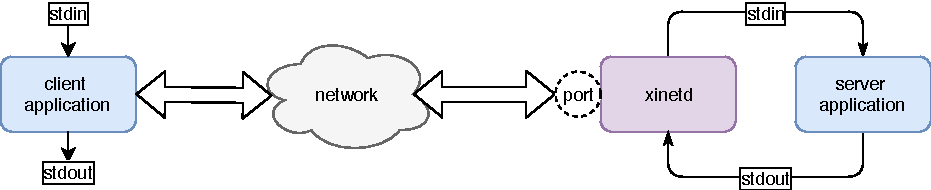
\includegraphics[scale=0.9]{figures/xinetd.pdf}
    \caption{xinetd socket activation}
    \label{fig_xinetd}
\end{figure}
xinetd features access control mechanisms such as TCP Wrapper ACLs (access control lists), extensive logging capabilities, and the ability to make services available based on time.
It can place limits on the number of servers that the system can spawn.
xinetd is listening on behalf of the services.
Whenever a connection would come in an instance of the respective service will be spawned with using {\it stdin} and {\it stdout} of the service application\cite{xinetd}.


\section{Package the Tang}
Similarly to José we need to create a new package for OpenWrt.
Let us create a branch and {\tt utils/tang} directory where binary programs like Tang belongs to:
\begin{lstlisting}[columns=fixed,basicstyle=\ttfamily\footnotesize,tabsize=4,backgroundcolor=\color{yellow!10}]
$ git chechout -b add-tang master
$ mkdir -p utils/tang/
\end{lstlisting}
The Tang project is owned by same owner on GitHub as José.
We should visit the project releases page\footnote{https://github.com/latchset/tang/releases/} and get the Tang version v6.
Then add following lines to the Makefile similarly as with José's Makefile:
\begin{lstlisting}[columns=fixed,basicstyle=\ttfamily\footnotesize,tabsize=4,backgroundcolor=\color{yellow!10}]
include $(TOPDIR)/rules.mk

PKG_NAME:=tang
PKG_VERSION:=6
PKG_RELEASE:=1

PKG_SOURCE:=$(PKG_NAME)-$(PKG_VERSION).tar.bz2
PKG_SOURCE_URL:=\
https://github.com/latchset/$(PKG_NAME)/releases/download/v$(PKG_VERSION)/

PKG_HASH:=1df78b48a52d2ca05656555cfe52bd4427c884f5a54a2c5e37a7b39da9e155e3


PKG_INSTALL:=1
PKG_BUILD_PARALLEL:=1

PKG_FIXUP:=autoreconf

include $(INCLUDE_DIR)/package.mk
\end{lstlisting}
Do not forget to add the package description which should have section dependencies filled.
\begin{itemize}
    \item libhttp-parser -- used for parsing HTTP requests.
    \item José -- the library and tool for the JavaScript Object Signing and Encryption.
    \item xinetd (a run-time dependency)
    \item bash (a run-time dependency)
\end{itemize}
The actual build proccess of the Tang does not require xinetd's libraries but will be configured to use its socket activation available in run-time.
The bash dependency is there for a reason that Tang's {\tt tangd-update} and {\tt tangd-keygen} executables are bash scripts.
These scripts are complex and are using data structures that are not available for OpenWrt's default shell - ash.
Having run-time dependencies listed in the Makefile will ensure that they are installed to the device before the Tang.
\begin{lstlisting}[columns=fixed,basicstyle=\ttfamily\footnotesize,tabsize=4,backgroundcolor=\color{yellow!10}]
define Package/tang
  SECTION:=utils
  TITLE:=tang v$(PKG_VERSION) - daemon for binding data to a third party
  DEPENDS:=+libhttp-parser +xinetd +jose +bash
  URL:=https://github.com/latchset/tang
endef
\end{lstlisting}
The Tang package will be present in utils section of the {\tt openwrt/packages} repository.
Let us add a brief description to our new package using description define:
\begin{lstlisting}[columns=fixed,basicstyle=\ttfamily\footnotesize,tabsize=4,backgroundcolor=\color{yellow!10}]
define Package/tang/description
	Tang is a small daemon for binding data to the presence of a third party
endef
\end{lstlisting}
The buildroot should know where to install the Tang's binaries.
Let us define a install section and use standard tangd binary location as on Fedora OS:
\begin{lstlisting}[columns=fixed,basicstyle=\ttfamily\footnotesize,tabsize=4,backgroundcolor=\color{yellow!10}]
define Package/tang/install
	$(INSTALL_DIR)	$(1)/usr/libexec
	$(INSTALL_BIN)	\
			$(PKG_INSTALL_DIR)/usr/lib/$(PKG_NAME)d*	$(1)/usr/libexec/
endef
\end{lstlisting}
Let us not forget the last line which allows the actual "magic" to happen:
\begin{lstlisting}[columns=fixed,basicstyle=\ttfamily\footnotesize,tabsize=4,backgroundcolor=\color{yellow!10}]
$(eval $(call BuildPackage,$(PKG_NAME)))
\end{lstlisting}
We can now merge these changes to feeds and try to build our freshly created Tang package:
\begin{lstlisting}[columns=fixed,basicstyle=\ttfamily\footnotesize,tabsize=4,backgroundcolor=\color{yellow!10}]
$ git commit -a
$ git push --set-upstream origin add-tang
$ git checkout new_pkgs
$ git merge add-tang
\end{lstlisting}
The new packagee tang will be available in the {\it Extra packages} section of the menuconfig after updating feeds:
\begin{lstlisting}[columns=fixed,basicstyle=\ttfamily\footnotesize,tabsize=4,backgroundcolor=\color{yellow!10}]
$ ./scripts/feeds update packages
$ ./scripts/feeds install tang
$ make menuconfig
$ make package/tang/{clean,compile}
\end{lstlisting}
After first try to build the tang package we will encounter the systemd dependency errror:
\begin{lstlisting}[columns=fixed,basicstyle=\ttfamily\footnotesize,tabsize=4,backgroundcolor=\color{yellow!10}]
configure: error: Package requirements (systemd) were not met:

No package 'systemd' found

Consider adjusting the PKG_CONFIG_PATH environment variable if you
installed software in a non-standard prefix.
\end{lstlisting}
We did not defined systemd dependency for Makefile but the cross-compilation of the package will try to configure and compile downloaded sources.
Compiler will try to find the systemd dependency as it is defined as dependency in the {\tt configure.ac} file in Tang repository.
We shall remove this builtime dependency.

To do so we will remove a requirement for systemd from the Tang's configure.ac and Makefile.am file.
These patches are too extensive to be demonstrated.
{\it Makefile\_am.patch} and {\it configure\_ac.patch} can be found in submitted pull-request files\footnote{https://github.com/openwrt/packages/pull/5447/files} on GitHub.

To have sources patched before compilation we have to crate a directory for them in the package's feeds repository we forked on branch containing commit adding the Tang and copy them to created directory:
\begin{lstlisting}[columns=fixed,basicstyle=\ttfamily\footnotesize,tabsize=4,backgroundcolor=\color{yellow!10}]
$ cd packages-OpenWrt
$ git checkout add-tang
$ mkdir -p utils/tang/patches
\end{lstlisting}
Patches included in this directory are automatically applied on the sources downloaded from the mirror in the build time.

To have these changes in our feeds in buildroot commit them and push to add-tang branch.
After these changes pushed and merged with {\it new\_pkgs} branch a rebuild of the tang package we will succeed.
Now we have Tang package ready to be installed on our device.

We are avoiding troubles with using the libhttp-parser in version 2.8.0.
These problems are described in following subsection \ref{porting_problems}.
The most important part after successful build would be to configure it correctly.



\subsection{Delivering Tang package}\label{porting_problems}

The upstream world is not always ideal.
Soon after this porting effort started OpenWrt upstream was in bad shape and almost dead for reasons we described in subsection \ref{LEDE} OpenWrt and LEDE.
The active part of OpenWrt developers decided to focus on LEDE project and submitting a pull-request to the OpenWrt was painful.
Working with outdated buildroot (or an SDK) was not ideal.
We decided to use upstream version of buildroot after re-merge.
It solved many issues with outdated dependencies that came into way.

\paragraph{Outdated buildroot} caused many issues with dependencies but as we installed older version of them the build could be triggered.
The most time consuming thing was to run build over and over and collect linker and compiler errors and adding additional flags into Makefile such as:
\begin{lstlisting}[columns=fixed,basicstyle=\ttfamily\footnotesize,tabsize=4,backgroundcolor=\color{yellow!10}]
+CFLAGS += -fhonour-copts
+TARGET_CFLAGS += $(FPIC) -std=gnu99
+TARGET_LDFLAGS += -Wl,-rpath-link=$(1)/usr/lib
\end{lstlisting}
Same flags and running build over an over were happening with José and with the Tang.
In case of Tang there was one additional TARGET\_CFLAGS option:
\begin{lstlisting}[columns=fixed,basicstyle=\ttfamily\footnotesize,tabsize=4,backgroundcolor=\color{yellow!10}]
-D_GNU_SOURCE
\end{lstlisting}
Without this option Tang was issuing a compilation errors with implicit declaration of the functions:
\begin{lstlisting}[columns=fixed,basicstyle=\ttfamily\footnotesize,tabsize=4,backgroundcolor=\color{yellow!10}]
dprintf()
vdprintf()
\end{lstlisting}
Using uptream buildroot solved these issues for good.

\paragraph{libhttp-parser} dependency has been in its latest version 2.7.1 when the effort started.
Unfortunately building the Tang package with libhttp-parser updated to version 2.7.1 failed on dependency and has thrown an error:
\begin{lstlisting}[columns=fixed,basicstyle=\ttfamily\footnotesize,tabsize=4,backgroundcolor=\color{yellow!10}]
checking for http_parser.h... no
configure: error: http-parser required!
\end{lstlisting}
We found out that Fedora's package http-parser contains one patch\footnote{https://github.com/nodejs/http-parser/pull/337} to add functionality required by the Tang to the http-parser.
Actual checking of the header was in configure.ac file of the Tang package:
\begin{lstlisting}[columns=fixed,basicstyle=\ttfamily\footnotesize,tabsize=4,backgroundcolor=\color{yellow!10}]
AC_CHECK_HEADER([http_parser.h], [],
		[AC_MSG_ERROR([http-parser required!])], [
#include <http_parser.h>
#ifndef HTTP_STATUS_MAP
#error HTTP_STATUS_MAP not defined!
#endif
])
\end{lstlisting}
We first considered applying the very same patch form Fedora package to the http-parser in version 2.7.1 in OpenWrt but in the end the release 2.8.0 solved the dependency error for a {\it HTTP\_STATUS\_MAP} macro.
On the other hand it brought another issue:
\begin{lstlisting}[columns=fixed,basicstyle=\ttfamily\footnotesize,tabsize=4,backgroundcolor=\color{yellow!10}]
Package tang is missing dependencies for the following libraries:
libhttp_parser.so.2.8
\end{lstlisting}
Adding a symbolic link to the libhttp-parser's install sections of the Makefile will suffice.
\begin{lstlisting}[columns=fixed,basicstyle=\ttfamily\footnotesize,tabsize=4,backgroundcolor=\color{yellow!10}]
ln -s libhttp_parser.so.$(PKG_VERSION) libhttp_parser.so.2.8
\end{lstlisting}

  \chapter{Configuring the Tang on OpenWrt}\label{config}

Having the installable packages in our buildroot is only the half of the work done.
We need to install them on the actual device and setup the environment especially for the Tang server to work correctly.
The installation of the packages on OpenWrt is done with the opkg package manager.

The opkg (Open Package Management System) is a lightweight package manager used to download and install OpenWrt packages.
These packages could be stored somewhere on device's file-system or the package manager will download them from local package repositories or ones located on the Internet mirrors.
Users already familiar with GNU/Linux package managers like dnf, yum, apt/apt-get, pacman, emerge etc. will recognize the similarities.
It also has similarities with NSLU2's Optware, also made for embedded devices.

Opkg attempts to resolve dependencies with packages in the available repositories/mirrors.
If the opkg fails to find the dependency, it will report an error, and abort the installation of selected package.

By removing systemd lines from sources we end up not have automatic updates of the Tang's cache and xinetd's socket activation to set up.



\section{Install the packages}

The packages that have been built in our buildroot are not available in any online mirror yet.
To make them available for OpenWrt we should create a pull-request tith the change and work with the community to accept it.
Before we do so, we have to make sure, that the built packages are working try installing them and testing their functionality.

To get our newly built packages to the target device running the OpenWrt we can upload them using scp to device's file-system.
After successful build, the packages are present in the bin/packages/mips\_24kc/packages/ directory (the location is bound to device configuration):
\begin{lstlisting}[columns=fixed,basicstyle=\ttfamily\footnotesize,tabsize=4,backgroundcolor=\color{yellow!10}]
$ scp bin/packages/mips_24kc/packages/*.ipk \
    root@192.168.0.1:/root/custom-packages/
\end{lstlisting}
This command will upload every package built before in builroot to the device's directory {\tt /root/custom-packages/}.
The buildroot should contain at least these files:
\begin{lstlisting}[columns=fixed,basicstyle=\ttfamily\footnotesize,tabsize=4,backgroundcolor=\color{yellow!10}]
$ ls bin/packages/mips_24kc/packages/
bash_4.4.12-1_mips_24kc.ipk
jansson_2.10-1_mips_24kc.ipk
jose_10-1_mips_24kc.ipk
libhttp-parser_2.8.0-1_mips_24kc.ipk
libjose_10-1_mips_24kc.ipk
Packages
Packages.gz
Packages.manifest
Packages.sig
tang_6-1_mips_24kc.ipk
xinetd_2.3.15-5_mips_24kc.ipk
\end{lstlisting}
After the successful upload, connect to the device and install packages.
We recommend installing only newly built or updated packages.
opkg will resolve known dependencies from the mirrors and will install them.
The {\tt /root/custom-pacakges} is not set up as custom opkg feed, thus we need to install tang and ist depencencies manually in order:
\begin{lstlisting}[columns=fixed,basicstyle=\ttfamily\footnotesize,tabsize=4,backgroundcolor=\color{yellow!10}]
opkg install /root/custom-packages/jansson_2.10-1_mips_24kc.ipk
opkg install /root/custom-packages/jose_10-1_mips_24kc.ipk
opkg install /root/custom-packages/libhttp-parser_2.8.0-1_mips_24kc.ipk
opkg install /root/custom-packages/tang_6-1_mips_24kc.ipk
\end{lstlisting}
The opkg tool will resolve other known dependencies and install them as well.
After packages are installed we may now proceed to the enviroment setup.



\section{Setting up the Tang keys}
The Tang server is packaged with cripts which help us to generate keys and cache for the Tang daemon.
OpenWrt has no realpath available, therefore the {\tt tangd-update} script did not work on OpenWrt.
\begin{lstlisting}[columns=fixed,basicstyle=\ttfamily\footnotesize,tabsize=4,backgroundcolor=\color{yellow!10}]
bash: realpath: command not found
\end{lstlisting}
Simply replacing it with {\tt readlink -f} solved the issue and script with such change is capable of generating cache.
We have to create a diff file for this change and add it into {\tt utils/tang/patches} directory.

The OpenWrt Makefile can define section {\it Package/\$(PKG\_NAME)/postinst}.
This section usually contain a short shell script to tweak the package after installation to make package work out of the box.
We can place this short sript to the Tang's Makefile to run the keys and cache generation after installation:
\begin{lstlisting}[columns=fixed,basicstyle=\ttfamily\footnotesize,tabsize=4,backgroundcolor=\color{yellow!10}]
define Package/tang/postinst
#!/bin/sh
if [ -z "$${IPKG_INSTROOT}" ]; then
	mkdir -p /usr/share/tang/db && mkdir -p /usr/share/tang/cache
	KEYS=$(find /usr/share/tang/db/ -name "*.jw*" -maxdepth 1 | wc -l)
	if [ "${KEYS}" = "0" ]; then # if db is empty generate new key pair
		/usr/libexec/tangd-keygen /usr/share/tang/db/
	elif [ "${KEYS}" = "1" ]; then # having 1 key should not happen
		(>&2 echo "Please check the Tang's keys in /usr/share/tang/db \
and regenate cache using /usr/libexec/tangd-update script.")
	else
		/usr/libexec/tangd-update /usr/share/tang/db/ /usr/share/tang/cache/
	fi
fi
endef
\end{lstlisting}



\section{Configure Tang for xinetd}

We need xinetd's socket activation for Tang to work.
And to do so we will need a configuration file for the tangd service for xinetd daemons shown in listing \ref{tangdx}.
\begin{lstlisting}[columns=fixed,basicstyle=\ttfamily\footnotesize,tabsize=4,backgroundcolor=\color{yellow!10},caption=Configuration of Tang service for xinetd,label=tangdx]
service tangd
{
    port            = 8888
    socket_type     = stream
    wait            = no
    user            = root
    server          = /usr/libexec/tangd
    server_args     = /usr/share/tang/cache
    log_on_success  += USERID
    log_on_failure  += USERID
    disable         = no
}
\end{lstlisting}
This is configuration to run {\tt /usr/libexec/tangd} after a request comes to port 8888.
The server will be spawned with one argument, the cache directory.
Please note that we used diffent directory compared to Fedora.
We need to have Tang keys stored on persistent data storage.
The {\tt /var/} location is only a symbolic link to the {\tt /tmp} directory on OpenWrt device.
The developers on IRC channel proposed to use the persistent {\tt /usr/share/} directory for that purpose.
The last step before starting the Tang service on OpenWrt would be to setup {\tt /etc/services}:
\begin{lstlisting}[columns=fixed,basicstyle=\ttfamily\footnotesize,tabsize=4,backgroundcolor=\color{yellow!10}]
# echo -e "tangd\t\t8888/tcp" >> /etc/services
\end{lstlisting}
and add the very same thing to post-installation script to have Tang completelly set up after installation:
\begin{lstlisting}[columns=fixed,basicstyle=\ttfamily\footnotesize,tabsize=4,backgroundcolor=\color{yellow!10}]
(cat /etc/services | grep -E "tangd.*8888\/tcp") > /dev/null \
    || echo -e "tangd\t\t8888/tcp" >> /etc/services
\end{lstlisting}
In case of the accidental removal of {\tt /etc/services} file we have to copy the backup of the file from devices ROM and edit it again.
\begin{lstlisting}[columns=fixed,basicstyle=\ttfamily\footnotesize,tabsize=4,backgroundcolor=\color{yellow!10}]
# cp /rom/etc/services /etc/services
\end{lstlisting}
Now we shall restart the xinetd daemon using the xinetd script located in {\tt /etc/init.d/} directory to enable tangd service using xinetd's socket activation:
\begin{lstlisting}[columns=fixed,basicstyle=\ttfamily\footnotesize,tabsize=4,backgroundcolor=\color{yellow!10}]
# /etc/init.d/xinetd stop
# /etc/init.d/xinetd start
\end{lstlisting}
To test that service is running we can use the telnet to the device on port defined in the xinetd configuration.
The server should advertise its public key.
It can be retrieved with simple {\it GET} request for {\it /adv} content from the server.
Try telnet to device write “GET /adv HTTP/1.1” and confirm this with two newlines (return key).
The output similar to following should appear:
\begin{lstlisting}[columns=fixed,basicstyle=\ttfamily\footnotesize,tabsize=4,backgroundcolor=\color{yellow!10}]
$ telnet 192.168.0.1 8888
Trying 192.168.0.1...
Connected to 192.168.0.1.
Escape character is '^]'.
GET /adv HTTP/1.1

<unknown> GET /adv => 200 (src/tangd.c:85)
HTTP/1.1 200 OK
Content-Type: application/jose+json
Content-Length: 956

{"payload":"eyJrZXlzIjpbeyJhbGciOiJFQ01SIiwiY3J2IjoiUC01MjEiLCJrZXlfb3BzIjpb
ImRlcml2ZUtleSJdLCJrdHkiOiJFQyIsIngiOiJBR3V2amxUZmpYaDBraWFEa19Tak1vMGhYUm1R
dzFZNkVkNE9yN3Fza2J2c1h6QUlvRTl5ZnRwR2xRVng1OVlxZ1gtR3hQSE8tdzVLVXFmanRGQkVV
ZVByIiwieSI6IkFiNE9NNTBhQ1Y4NkdZVW1PdHBua1VTanNXNUFleENXZG5PZFEyakl0Z1RGNXNq
MG1TSFZCYXhsd2w1N3ZTUEdrSExiRl96SFlUVzlvVzNoTFJyeXRRNmYifSx7ImFsZyI6IkVTNTEy
IiwiY3J2IjoiUC01MjEiLCJrZXlfb3BzIjpbInZlcmlmeSJdLCJrdHkiOiJFQyIsIngiOiJBQVpS
ZmNlNUhLaFYyck1OQzhqLW5iVW1pdlh4NDRjcU1qX2Jvbk5OdnNTcXdBRjhFcGoyTFM0cFpfdUNR
VDJGVDRUSHJnX1Y4VHBKci1PQW41Z05CaUZNIiwieSI6IkFTMjJSdVJZZXVOU1ZtSkdfSmcwSW1n
by1LREd2QVFPZV9Vdk9fT3RZS3lGeUVoSWI1U0FLd3cwSEF0QjJFX2FTMG5pcWV3UUlod1QyanR5
eklCaWdkQU0ifV19","protected":"eyJhbGciOiJFUzUxMiIsImN0eSI6Imp3ay1zZXQranNvb
iJ9","signature":"ADpGOjYeB45MznQOxA6Pw9MXTMYQ649UkRSi_RsP8KPKosl-eA7GmOIiBM
FOoPnCNX-cGjhyDBbQuvESUCJ_3txjANf-srntxFAX5p72Eip-kROGrlCdLrVLnlg36itQUBFx7S
UyB_7I6CX6gdpWyJ-wtro8f2Snu6wwMGl-8V3ylWYr"}
\end{lstlisting}
The content of the first line from server response should be suspicious to us.
According to the RFC 2616 the HTTP header should not contain such line\cite{RFC2616}.
\begin{lstlisting}[columns=fixed,basicstyle=\ttfamily\footnotesize,tabsize=4,backgroundcolor=\color{yellow!10}]
<unknown> GET /adv => 200 (src/tangd.c:85)
\end{lstlisting}
After some investigation done in the Tang sources we found out that the line contains debug information from the Tang daemon which were written to the /dev/stderr.
From this we can assume that xinetd is sending also {\tt /dev/stderr} to the network socket.
To bypass this beavior we should write wrapper script which will redirect the {\tt /dev/stderr} output somewhere else.
We decided that this output may be helpful for debugging purpose and forwarded it to the log file in the {\tt /var/log/} directory of the device using this script:
\begin{lstlisting}[columns=fixed,basicstyle=\ttfamily\footnotesize,tabsize=4,backgroundcolor=\color{yellow!10}]
#!/bin/bash
echo "==================================" >> /var/log/tangd.log
echo `date`: >> /var/log/tangd.log
/usr/libexec/tangd $1 2>> /var/log/tangd.log
\end{lstlisting}
Let us name this wrapper script the tangdw.

To get Tang to work we need to put invocation of this script in place where tangd binary was configured to.
Move the script to the /usr/libexec directory where the tangd binary is to have it in one place and edit the line of xinetd configuration to run wrapper:
\begin{lstlisting}[columns=fixed,basicstyle=\ttfamily\footnotesize,tabsize=4,backgroundcolor=\color{yellow!10}]
    server          = /usr/libexec/tangdw
\end{lstlisting}
The last thing would be to change the script's permissions on device to allow execution.

We did a lot changes to the configuration.
The Tang for the OpenWrt platform needs a xinetd configuration which for the ease of use could be packaged with it.
The same with the wrapper script in order to have the service working correctly we also need this file.
There is a way to add new files for each package and package them for the OpenWrt's opkg to install.
To do so we will crate a directory for the files in the package's feeds repository we forked on branch containing commit adding the Tang and copy files there.
\begin{lstlisting}[columns=fixed,basicstyle=\ttfamily\footnotesize,tabsize=4,backgroundcolor=\color{yellow!10}]
$ cd packages-OpenWrt
$ git checkout add-tang
$ mkdir -p utils/tang/files
\end{lstlisting}
As the new files are copied there we need to also edit a {\it Package/tang/install} section to install these files in proper directories (config file into dedicated {\tt /etc/xinetd.d/}; wrapper into {\tt /usr/libexec/}) as shown:\newpage
\begin{lstlisting}[columns=fixed,basicstyle=\ttfamily\footnotesize,tabsize=4,backgroundcolor=\color{yellow!10}]
define Package/tang/install
	$(INSTALL_DIR)	$(1)/usr/libexec
	$(INSTALL_DIR)	$(1)/etc/xinetd.d/
	$(INSTALL_BIN)	\
			$(PKG_INSTALL_DIR)/usr/libexec/$(PKG_NAME)d*  $(1)/usr/libexec/
	$(INSTALL_BIN)	./files/tangdw	$(1)/usr/libexec/
	$(CP)			./files/tangdx	$(1)/etc/xinetd.d/
endef
\end{lstlisting}
After all changes done last, we need to to amend commit on a branch, update the feeds in buildroot, rebuild the Tang package, upload and re-install it on our device running the OpenWrt.
Due to many changes to the Makefile and the Tang branch in packages see the submitted pull-request\footnote{https://github.com/openwrt/packages/pull/5447} which includes all the changes.



\section{Tang's limitations}\label{limitations}

Let us sum up the limitations that Tang has on OpenWrt platform due to replaced systemd dependency with less capable xinetd implementation of super-server.
We also found one platform independent limitation of the Tang's solution to full disk description on early boot.

\paragraph{Key exchange and generation} of cache must be manual but  can be automated with inotifytools to watch directory for change and run update script automatically.
But this mean that the embedded device with such configuration will have another process always running.
We decided to not implement automated update of the cache to save the computation resources.

\paragraph{xinetd forwarding the stderr} output to the socket as well is a little problem.
To have tang working correctly we wrote a wrapper running the shell script redirecting the {\it stderr} into log file.
Running some shell script takes some time compared to only running the binary file but for xinetd it is necessary.

\paragraph{Early boot decryption using Wi-Fi network} is a platform independent chicken-egg problem caused by information about wireless network being encrypted on system volume.
The information needed to connect to wireless network needs to be decrypted but in order to decrypt them automatically we need to connect to network exposed to Tang server.
It could be solved using a TPM to store information about such network but it is a security vulnerability and must be considered with a caution.

  \chapter{Conclusion}\label{conlusion}



The Tang \ref{tang} server is a very lightweight program.
It provides secure and anonymous data binding using McCallum-Relyea exchange \ref{mrexchange} algorythm.

As every server purpose is to serve its clients, it needs to have client application.
In case of Tang we have Clevis.
Clevis \ref{clevis} is a client software with full support for Tang.
It has minimal dependencies and it is possible to use with HTTP, Escrow \ref{escrow}, and it implements Shamir Secret Sharing.
Clevis has GNOME integration so it is not only a command line tool.
Clevis also supports removable devices unocking using UDisks2 or even early boot integration with dracut, which was this thesis inspiration and goal to achieve with only embedded device supported OpenWrt running Tang server.

To port Tang to OpenWrt system it was necesarry to port all its dependencies first.
The OpenWrt system has already package openssl, zlib, and jansson but only version 2.7 which was too old.
So there was a need for updating jansson to resolve all dependencies for package José.
José required porting and after focusing on upstream version porting on this package was straightforward.
After struggling with older version, package http-parser known as libhttp-parser in OpenWrt feeds, is now updated to latest upstream version 2.8.0.
The systemd would be huge effort but tang's requirements are minimal and we were able to work with xinetd's socket activation.
With correct configuration of xinetd and removing dependency for systemd Tang server is running on OpenWrt with some platform specific changes mentioned in chapter \ref{porting-tang} Porting Tang.


  % Kompilace po částech (viz výše, nutno odkomentovat)
  % Compilation piecewise (see above, it is necessary to uncomment it)
  %\subfile{projekt-01-uvod-introduction}
  % ...
  %\subfile{chapters/xdudla00-porting-Tang-to-Open-WRT-01-introduction}
  %\subfile{chapters/xdudla00-porting-Tang-to-Open-WRT-02-encryption}
  %\subfile{ ... Add if required}

  % Pouzita literatura / Bibliography
  % ----------------------------------------------
\ifslovak
  \makeatletter
  \def\@openbib@code{\addcontentsline{toc}{chapter}{Literatúra}}
  \makeatother
  \bibliographystyle{bib-styles/czechiso}
\else
  \ifczech
    \makeatletter
    \def\@openbib@code{\addcontentsline{toc}{chapter}{Literatura}}
    \makeatother
    \bibliographystyle{bib-styles/czechiso}
  \else
    \makeatletter
    \def\@openbib@code{\addcontentsline{toc}{chapter}{Bibliography}}
    \makeatother
    \bibliographystyle{bib-styles/englishiso}
  %  \bibliographystyle{alpha}
  \fi
\fi
  \begin{flushleft}
  \bibliography{bibl/xdudla00-porting-Tang-to-Open-WRT-20-bibliography,bibl/bibl_rfc_1-3826,bibl/bibl_rfc_3826-7736}
  \end{flushleft}

  % vynechani stranky v oboustrannem rezimu
  % Skip the page in the two-sided mode
  \iftwoside
    \cleardoublepage
  \fi

  % Prilohy / Appendices
  % ---------------------------------------------
  \appendix
\ifczech
  \renewcommand{\appendixpagename}{Přílohy}
  \renewcommand{\appendixtocname}{Přílohy}
  \renewcommand{\appendixname}{Příloha}
\fi
\ifslovak
  \renewcommand{\appendixpagename}{Prílohy}
  \renewcommand{\appendixtocname}{Prílohy}
  \renewcommand{\appendixname}{Príloha}
\fi
%  \appendixpage

% vynechani stranky v oboustrannem rezimu
% Skip the page in the two-sided mode
%\iftwoside
%  \cleardoublepage
%\fi

\ifslovak
%  \section*{Zoznam príloh}
%  \addcontentsline{toc}{section}{Zoznam príloh}
\else
  \ifczech
%    \section*{Seznam příloh}
%    \addcontentsline{toc}{section}{Seznam příloh}
  \else
%    \section*{List of Appendices}
%    \addcontentsline{toc}{section}{List of Appendices}
  \fi
\fi
  \startcontents[chapters]
  \setlength{\parskip}{0pt}
  % seznam příloh / list of appendices
  % \printcontents[chapters]{l}{0}{\setcounter{tocdepth}{2}} % FIXME

  \ifODSAZ
    \setlength{\parskip}{0.5\bigskipamount}
  \else
    \setlength{\parskip}{0pt}
  \fi

  % vynechani stranky v oboustrannem rezimu
  \iftwoside
    \cleardoublepage
  \fi

  % Přílohy / Appendices
  % ----------------------------------------------
  \chapter{Compact disk content}
\begin{lstlisting}[columns=fixed,basicstyle=\ttfamily\footnotesize,tabsize=4]
a   -   b   -   d
    |       |
    |       -   e
    |
    -   c
\end{lstlisting}

  \chapter{Pre-installation enablement of hard drive encryption}
\label{luksinstall}

\section{Fedora 28 -- disc encryption option selecting }

\begin{figure}[h]
    \centering
    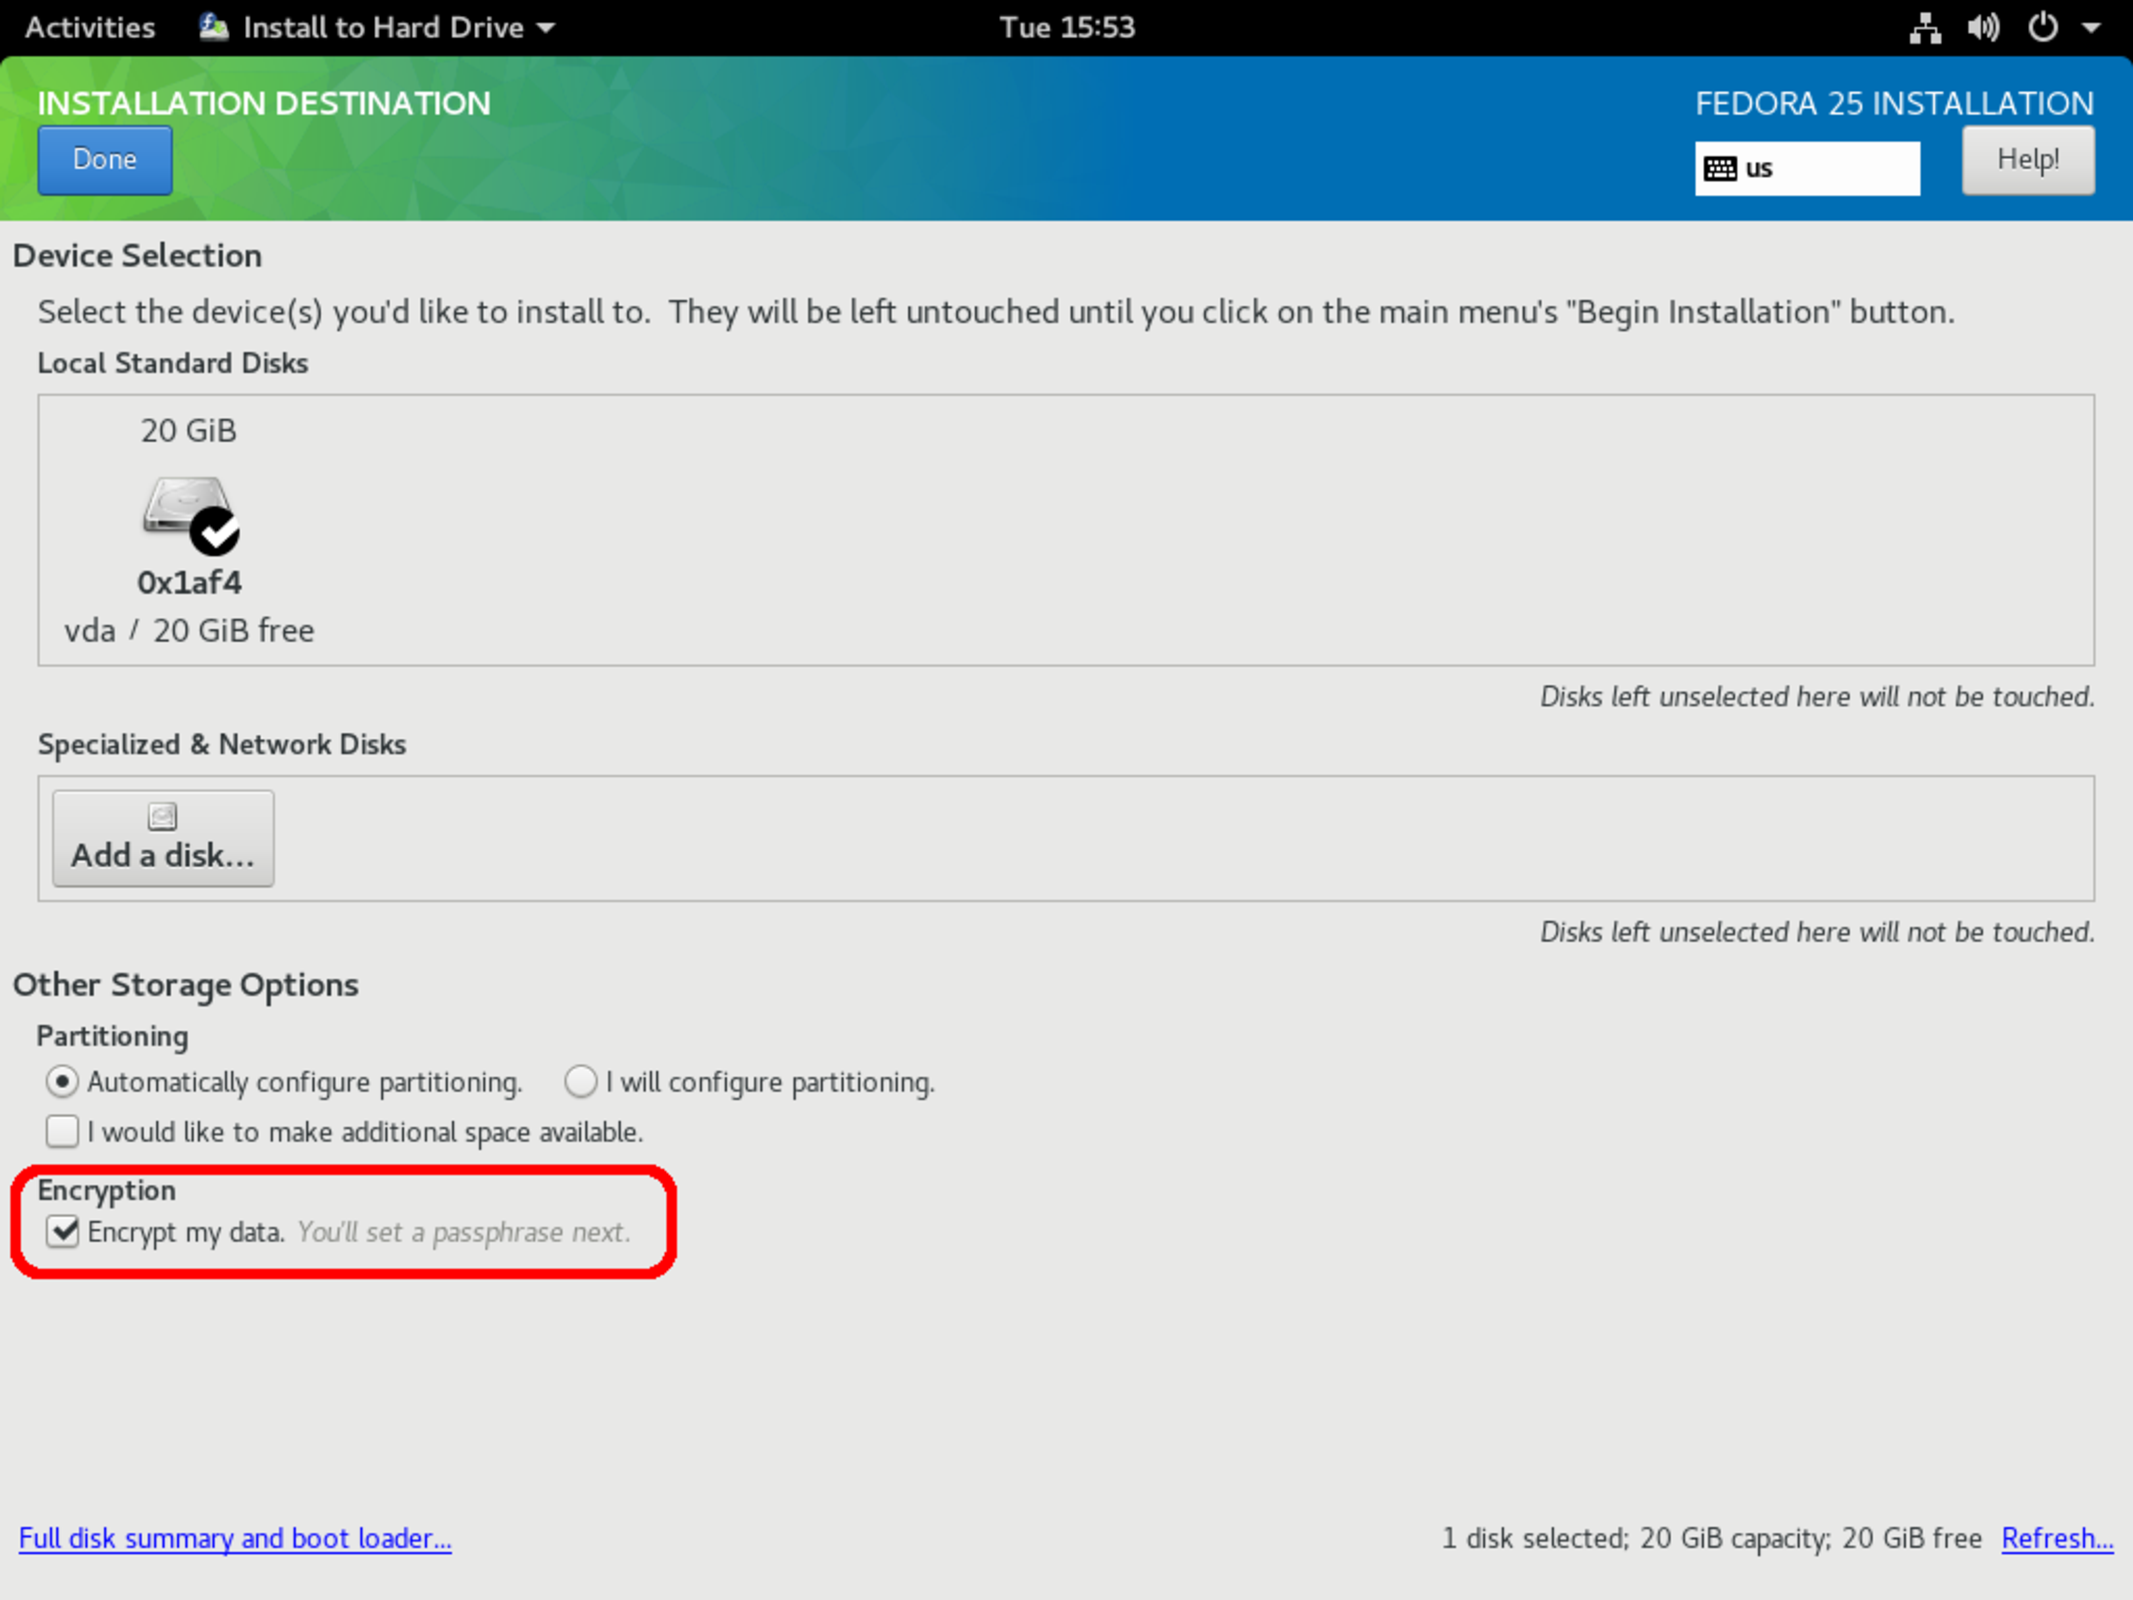
\includegraphics[scale=0.42]{figures/FedoraInstall1.pdf}
    \caption{Checking option}
\end{figure}

\newpage

\section{Fedora 28 -- determination key encryption key }

\begin{figure}[h]
    \centering
    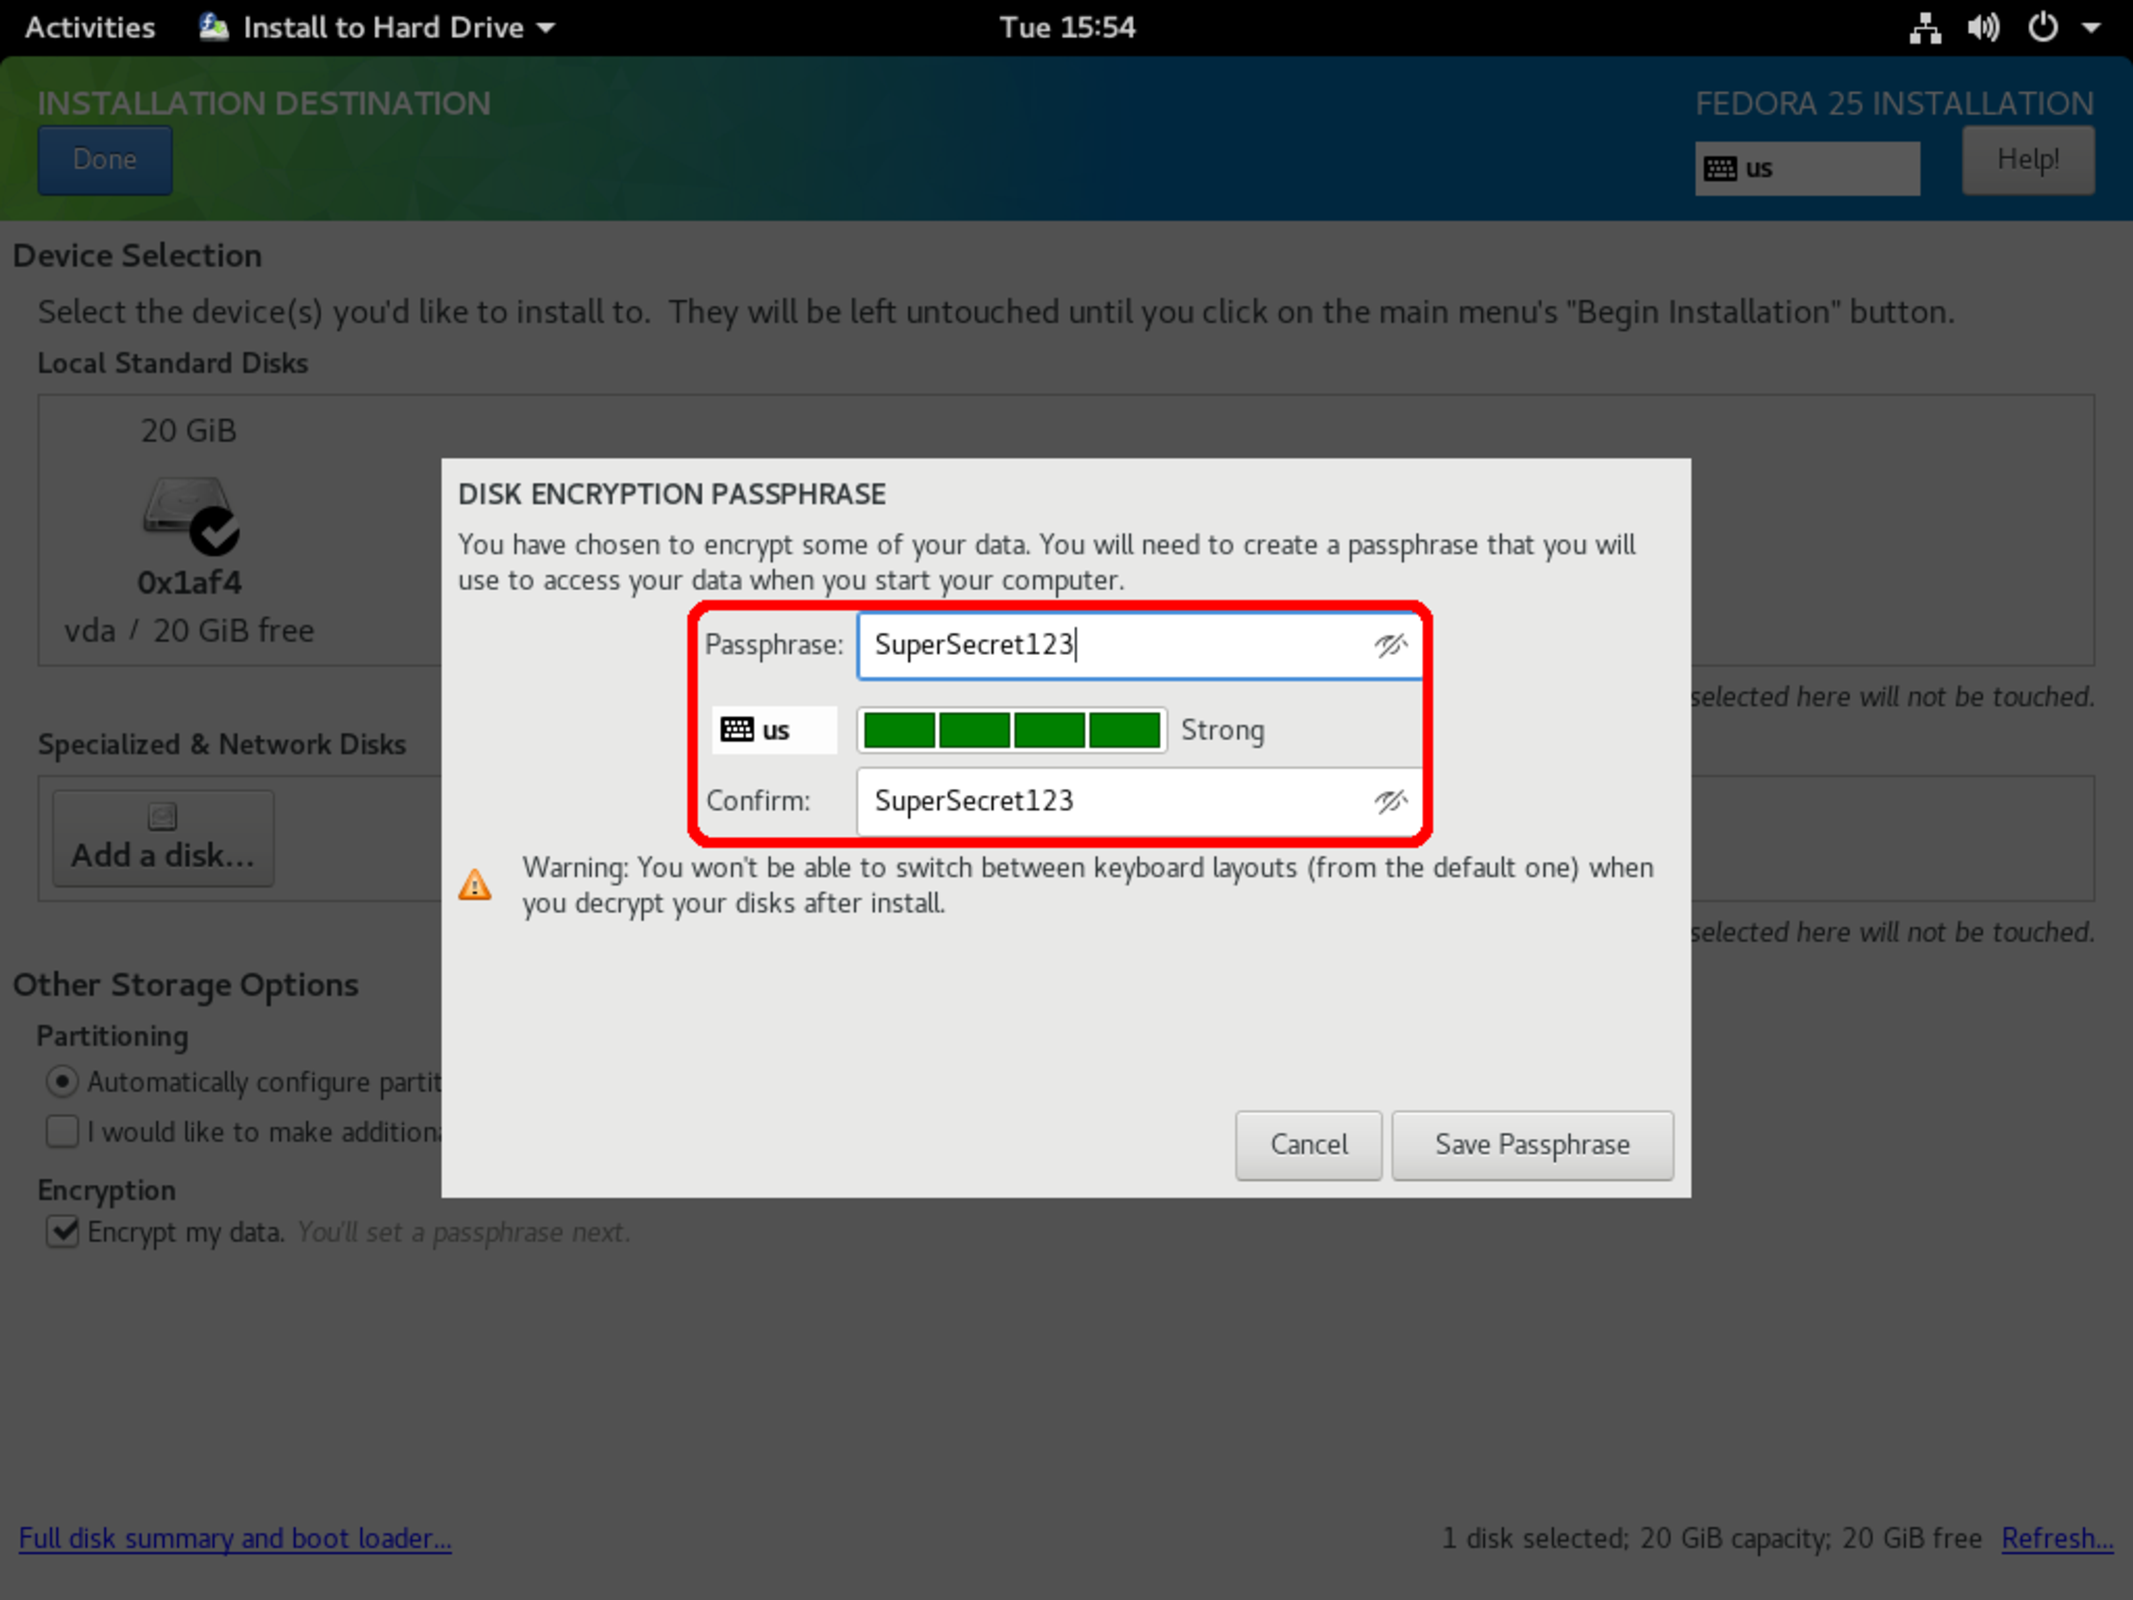
\includegraphics[scale=0.42]{figures/FedoraInstall2.pdf}
    \caption{Determining key}
\end{figure}

  \chapter{LUKS In-Place Encryption}
\label{luksipc}
It takes 4 steps to perform an in place encryption with {\it luksipc} \cite{luksipc}:
\begin{enumerate}
    \item Unmounting the filesystem
    \item Resizing the filesystem to shrink about 10 megabytes (2048 kB is the current LUKS header size -- but do not trust this value, it has changed in the past!)
    \item Performing luksipc
    \item Adding custom keys to the LUKS key-ring
\end{enumerate}



\paragraph{Step 1 -- Unmounting}
There should not be any problems unmounting partition, unless you want to encrypt {\it /} -- the root partition, which in our case (to lock whole disk) will be necessary.
To do so we need to restart our computer and boot any other or live distribution capable of completing these next steps.
\begin{lstlisting}[columns=fixed,basicstyle=\ttfamily\footnotesize,tabsize=4,backgroundcolor=\color{yellow!10}]
# umount /dev/vda2
\end{lstlisting}



\paragraph{Step 2 -- Resizing}
There are plenty tools for re-sizing, essentially for partitioning as whole (fdisk, e2fsck, etc.).
Demonstrating how this is done for ext 2, 3, 4 here:
\begin{lstlisting}[columns=fixed,basicstyle=\ttfamily\footnotesize,tabsize=4,backgroundcolor=\color{yellow!10}]
# e2fsck /dev/vda2
# resize2fs /dev/vda2 -s -10M
\end{lstlisting}
Delete and recreate shrank partition with fdisk:
\begin{lstlisting}[columns=fixed,basicstyle=\ttfamily\footnotesize,tabsize=4,backgroundcolor=\color{yellow!10}]
# fdisk /dev/vda
Welcome to fdisk (util-linux 2.23.2).

Changes will remain in memory only, until you decide to write them.
Be careful before using the write command.

Command (m for help):
\end{lstlisting}
Check the partition number with typing the {\tt p}:
\begin{lstlisting}[columns=fixed,basicstyle=\ttfamily\footnotesize,tabsize=4,backgroundcolor=\color{yellow!10}]
Command (m for help): p
Disk /dev/vda: 407.6 GiB, 437629485056 bytes, 854745088 sectors
Units: sectors of 1 * 512 = 512 bytes
Sector size (logical/physical): 512 bytes / 4096 bytes
I/O size (minimum/optimal): 4096 bytes / 4096 bytes
Disklabel type: dos
Disk identifier: 0x5c873cba
Partition 2 does not start on physical sector boundary.

Device        Boot        Start     End         Blocks      Id    System
/dev/vda1      *          2048      1026047     512000      83    Linux
/dev/vda2                 1026048   1640447     307200      8e    Linux LVM}
\end{lstlisting}



\paragraph{Step 3 -- Encrypting}
After this, luksipc comes into play. It performs an in-place encryption of the data and prepends the partition with a LUKS header. Firt we have to download luksipc or install it with package manager.
\begin{lstlisting}[columns=fixed,basicstyle=\ttfamily\footnotesize,tabsize=4,backgroundcolor=\color{yellow!10}]
$ wget https://github.com/johndoe31415/luksipc/archive/master.zip
$ unzip master.zip
$ cd luksipc-master/
$ make
\end{lstlisting}
Now run it with parameters like:
\begin{lstlisting}[columns=fixed,basicstyle=\ttfamily\footnotesize,tabsize=4,backgroundcolor=\color{yellow!10}]
# ./luksipc -d /dev/vda2
\end{lstlisting}
luksipc will have created a key file /root/initial\_keyfile.bin that you can use to gain access to the newly created LUKS device:
\begin{lstlisting}[columns=fixed,basicstyle=\ttfamily\footnotesize,tabsize=4,backgroundcolor=\color{yellow!10}]
# cryptsetup luksOpen --key-file /root/initial\_keyfile.bin \
    /dev/vda2 fedoradrive
\end{lstlisting}



\paragraph{Step 4 -- Adding key}
DO NOT FORGET to add key to LUKS volume:
\begin{lstlisting}[columns=fixed,basicstyle=\ttfamily\footnotesize,tabsize=4,backgroundcolor=\color{yellow!10}]
# cryptsetup luksAddKey --key-file /root/initial\_keyfile.bin /dev/vda2
\end{lstlisting}

  \chapter{Setting up the repository}\label{set_repo}

To save our work progress and be able to contribute to the upstream repository we should have a own fork of it.
A fork is a copy of a repository that we can manage.
It lets us make changes to a project without affecting the original (upstream) repository.
We can fetch updates from the upstream or submit changes to the original repository with pull requests.
These pull request are generated from the "devel" branch that we should have in our fork.

To fork OpenWrt's buildroot we should have our GitHub account set up\footnote{https://github.com/join}, visit the OpenWrt's project upstream repository\footnote{https://github.com/openwrt/openwrt}, and click on "Fork" button in the top-right corner of the page.
Before cloning our fork it is recommended to set up git enviroment\footnote{https://git-scm.com/book/en/v2/Getting-Started-First-Time-Git-Setup} on host machine and upload the SSH keys\footnote{https://help.github.com/articles/adding-a-new-ssh-key-to-your-github-account/} to our account to minimize pushing effort to our fork.
All work related to this thesis has been done using GitHub account Tiboris\footnote{https://github.com/Tiboris/} therefore output of following commands are bound to it.
\begin{lstlisting}[columns=fixed,basicstyle=\ttfamily\footnotesize,basicstyle=\ttfamily\footnotesize,tabsize=4,backgroundcolor=\color{yellow!10}]
$ git clone https://github.com/Tiboris/openwrt.git ~/buildroot-openwrt
\end{lstlisting}
Please note that this command will clone the {\it openwrt} repository of the GitHub user {\it Tiboris} to the {\it $\sim$/buildroot-openwrt} directory on our host.

To catch up with changes made upstream we should consider to configure a remote that points to it.
Configured remote allows us to sync changes made in the original repository with the fork and vice versa.
Make sure you are in the buildroot directory and add remote\footnote{https://help.github.com/articles/configuring-a-remote-for-a-fork/} called upstream:
\begin{lstlisting}[columns=fixed,basicstyle=\ttfamily\footnotesize,basicstyle=\ttfamily\footnotesize,tabsize=4,backgroundcolor=\color{yellow!10}]
$ cd ~/buildroot-openwrt
$ git git remote add upstream \
     https://github.com/openwrt/openwrt.git
\end{lstlisting}
To verify that remote is present run:
\begin{lstlisting}[columns=fixed,basicstyle=\ttfamily\footnotesize,basicstyle=\ttfamily\footnotesize,tabsize=4,backgroundcolor=\color{yellow!10}]
$ git remote -v
origin	git@github.com:Tiboris/openwrt.git (fetch)
origin	git@github.com:Tiboris/openwrt.git (push)
upstream	https://github.com/openwrt/openwrt.git (fetch)
upstream	https://github.com/openwrt/openwrt.git (push)
\end{lstlisting}
With the remote configured correctly we can now sync with
 upstream repository.
To download latest upstream changes use the "fetch" option
 and  the "merge" option to apply them to our fork's branch\footnote{https://help.github.com/articles/syncing-a-fork/}.
\begin{lstlisting}[columns=fixed,basicstyle=\ttfamily\footnotesize,basicstyle=\ttfamily\footnotesize,tabsize=4,backgroundcolor=\color{yellow!10}]
$ git fetch upstream master
remote: Counting objects: 4376, done.
remote: Compressing objects: 100% (2/2), done.
remote: Total 4376 (delta 1776), reused 1775 (delta 1775),
 pack-reused 2599
Receiving objects: 100% (4376/4376), 1.27 MiB
 | 743.00 KiB/s, done.
Resolving deltas: 100% (2932/2932), completed
 with 809 local objects.
From https://github.com/openwrt/openwrt
 * branch                  master     -> FETCH_HEAD
   36fb0697e2..d089a5d773  master     -> upstream/master
$ git merge upstream/master
\end{lstlisting}
The detailed description can be found on original GitHub pages\footnote{https://help.github.com/articles/working-with-forks/}.

  \chapter{Example OpenWrt package's Makefile}\label{hello_mkfile}
This is an example of what OpenWrt Makefile for package could look like.
The following makefile is slightly edited makefile from the tutorial\footnote{https://www.gargoyle-router.com/old-openwrt-coding.html} on the web.
\begin{lstlisting}[language=bash,basicstyle=\ttfamily\footnotesize,caption=Makefile for Helloworld.]
##############################################
# OpenWrt Makefile for helloworld program
#
#
# Most of the variables used here are defined in
# the include directives below. We just need to
# specify a basic description of the package,
# where to build our program, where to find
# the source files, and where to install the
# compiled program on the router.
#
# Be very careful of spacing in this file.
# Indents should be tabs, not spaces, and
# there should be no trailing whitespace in
# lines that are not commented.
#
##############################################

include $(TOPDIR)/rules.mk

# Name and release number of this package
PKG_NAME:=helloworld
PKG_RELEASE:=1

# This specifies the directory where we're going to build the program.
# The root build directory, $(BUILD_DIR), is by default the build_mipsel
# directory in your OpenWrt SDK directory
PKG_BUILD_DIR := $(BUILD_DIR)/$(PKG_NAME)

include $(INCLUDE_DIR)/package.mk

# Specify package information for this program.
# The variables defined here should be self explanatory.
# If you are running Kamikaze, delete the DESCRIPTION
# variable below and uncomment the Kamikaze define
# directive for the description below
define Package/helloworld
	SECTION:=utils
	CATEGORY:=Utilities
	TITLE:=Helloworld -- prints a snarky message
endef

# Uncomment portion below for Kamikaze and delete DESCRIPTION variable above
define Package/helloworld/description
	If you can't figure out what this program does, you're probably
	brain-dead and need immediate medical attention.
endef

# Specify what needs to be done to prepare for building the package.
# In our case, we need to copy the source files to the build directory.
# This is NOT the default.  The default uses the PKG_SOURCE_URL and the
# PKG_SOURCE which is not defined here to download the source from the web.
# In order to just build a simple program that we have just written, it is
# much easier to do it this way.
define Build/Prepare
	mkdir -p $(PKG_BUILD_DIR)
	$(CP) ./src/* $(PKG_BUILD_DIR)/
endef

# We do not need to define Build/Configure or Build/Compile directives
# The defaults are appropriate for compiling a simple program such as this one

# Specify where and how to install the program. Since we only have one file,
# the helloworld executable, install it by copying it to the /bin directory on
# the router. The $(1) variable represents the root directory on the router running
# OpenWrt. The $(INSTALL_DIR) variable contains a command to prepare the install
# directory if it does not already exist.  Likewise $(INSTALL_BIN) contains the
# command to copy the binary file from its current location (in our case the build
# directory) to the install directory.
define Package/helloworld/install
	$(INSTALL_DIR) $(1)/bin
	$(INSTALL_BIN) $(PKG_BUILD_DIR)/helloworld $(1)/bin/
endef

# This line executes the necessary commands to compile our program.
# The above define directives specify all the information needed, but this
# line calls BuildPackage which in turn actually uses this information to
# build a package.
$(eval $(call BuildPackage,helloworld))
\end{lstlisting}

  \chapter{List of pull-requests}\label{diffs}
Here is a list of all pull requests realated to the Tang porting effort.

\paragraph{package zlib}

Created pull-request that was not relevant because of zlib located in main OpenWrt repository see:

\begin{lstlisting}[columns=fixed,basicstyle=\ttfamily\footnotesize,tabsize=4,backgroundcolor=\color{yellow!10}]
https://github.com/openwrt/packages/pull/4290/files
\end{lstlisting}

\paragraph{package jansson}

Update of the package jansson was successful and merged upstrem in pull request:

\begin{lstlisting}[columns=fixed,basicstyle=\ttfamily\footnotesize,tabsize=4,backgroundcolor=\color{yellow!10}]
https://github.com/openwrt/packages/pull/4289/files
\end{lstlisting}

\paragraph{package libhttp-parser}

This pull request was not relevant and not merged because of http-parser already been located in packages repository under name libhttp-parser:

\begin{lstlisting}[columns=fixed,basicstyle=\ttfamily\footnotesize,tabsize=4,backgroundcolor=\color{yellow!10}]
https://github.com/openwrt/packages/pull/4304/files
\end{lstlisting}

Closed and not merged due to another pull request merged with bump into same version but without upstream patch containing HTTP\_STATUS\_MAP macro:
\begin{lstlisting}[columns=fixed,basicstyle=\ttfamily\footnotesize,tabsize=4,backgroundcolor=\color{yellow!10}]
https://github.com/openwrt/packages/pull/4335/files
\end{lstlisting}

Sucessfully merged bump into libhttp-parser version 2.8.0 containing the upstrem patch with HTTP\_STATUS\_MAP macro:
\begin{lstlisting}[columns=fixed,basicstyle=\ttfamily\footnotesize,tabsize=4,backgroundcolor=\color{yellow!10}]
https://github.com/openwrt/packages/pull/5446/files
\end{lstlisting}


\paragraph{package jose}

Still open (not merged yet) and waiting for review (12th May 2018):
\begin{lstlisting}[columns=fixed,basicstyle=\ttfamily\footnotesize,tabsize=4,backgroundcolor=\color{yellow!10}]
https://github.com/openwrt/packages/pull/4334/files
\end{lstlisting}


\paragraph{package tang}
Still open (not merged yet) and waiting for review (12th May 2018):
\begin{lstlisting}[columns=fixed,basicstyle=\ttfamily\footnotesize,tabsize=4,backgroundcolor=\color{yellow!10}]
https://github.com/openwrt/packages/pull/5447/files
\end{lstlisting}

  %\input{chapters/xdudla00-porting-Tang-to-Open-Wrt-Appendix-G}
  % ----------------------------------------------

  % kompilace po částech (viz výše, nutno odkomentovat)
  % compilation piecewise (see above, it is necessary to uncomment it)
%  \subfile{chapters/xdudla00-porting-Tang-to-Open-Wrt-Appendix-A}
%  \subfile{chapters/xdudla00-porting-Tang-to-Open-Wrt-Appendix-B}
%  \subfile{chapters/xdudla00-porting-Tang-to-Open-Wrt-Appendix-C}

\end{document}
